\documentclass[article,dr=phil,type=msc ,colorback,accentcolor=tud4b]{tudthesis}
\usepackage[ngerman,english]{babel}
\useshorthands{"}
\addto\extrasenglish{\languageshorthands{ngerman}}
\usepackage[scaled]{uarial}
\usepackage{amsmath}
\usepackage{enumitem}
\usepackage{epsfig}
\usepackage[outdir=./]{epstopdf}
\newcommand{\getmydate}{%
  \ifcase\month%
    \or Januar\or Februar\or M\"arz%
    \or April\or Mai\or Juni\or Juli%
    \or August\or September\or Oktober%
    \or November\or Dezember%
  \fi\ \number\year%
}
 
\begin{document}
  \thesistitle{Distributed Virtual Network Embedding without Sharing Topology Details}%
    {}
  \author{Tejamurthy Shivakumar}
  \birthplace{Darmstadt}
  \referee{Prof. Dr. Patrick Eugster}{M.Sc. Patrick Jahnke} 
  \department{Department of Computer Science}
  \group{Distributed Systems Programming}
  \dateofexam{\today}{\today}
  \tuprints{12345}{1234}
  \makethesistitle
  \affidavit{Tejamurthy Shivakumar}
  \setcounter{page}{0}
\tableofcontents


\newpage

 \section{Introduction}
 
Internet has been a huge success with its variety of applications and services contributing positively to the change, the world is witnessing today. Billions of connected devices and thousands of heterogeneous services running on the devices have challenged the performance of existing carrier networks. Current carrier networks are proprietary network infrastructures belonging to a telecommunications service provider which are not fully designed to handle the increase in traffic. In order to meet the diversified requirements of next-generation services and to be compatible with different levels of Quality of Service (QoS) demands by end users, traditional network architecture needs major changes. Researchers are focused on designing a new architecture for the future internet to address the challenges faced by existing Internet \cite{ 4086425}. \newline
 
 Alternative solution to the future internet is to accommodate multiple generations of mobile network in a same shared network substrate. This network sharing \cite{nw_sharing} solution although minimize the network cost, but has limitations in the field of network management such as: 1) Traffic isolation: clear separation between multiple networks' traffic. 2) Cross-domain Sharing: to share resources across multiple technology domains. 3) Monitoring: performance of each network needs to be monitored after its creation. 4) Dynamic sharing: automated dynamic resource sharing and 5) Security: Security for each network.\newline 
 
Designing a new architecture for future carrier networks overcomes the resistance of existing Internet to its architectural changes and is the main need of the time. Future Carrier Networks (FCN) should be able to scale billions of interconnected devices with thousands of heterogeneous services running on the network. The main challenges of FCNs [2] are to achieve service flexibility in order to adaptively provide a wide range of network services to each customer and to support applications with different levels of network QoS. Other research issues with FCNs include infrastructure sharing, optimal resource utilization and performance guarantees which needs more focus. Several ideas have been proposed to address these research challenges in order to design a new Internet architecture. Figure 1 shows proposed Future Internet Architecture from the book \cite{fcn_arc}. 
 
  \begin{figure}[h]
 	\centering
 	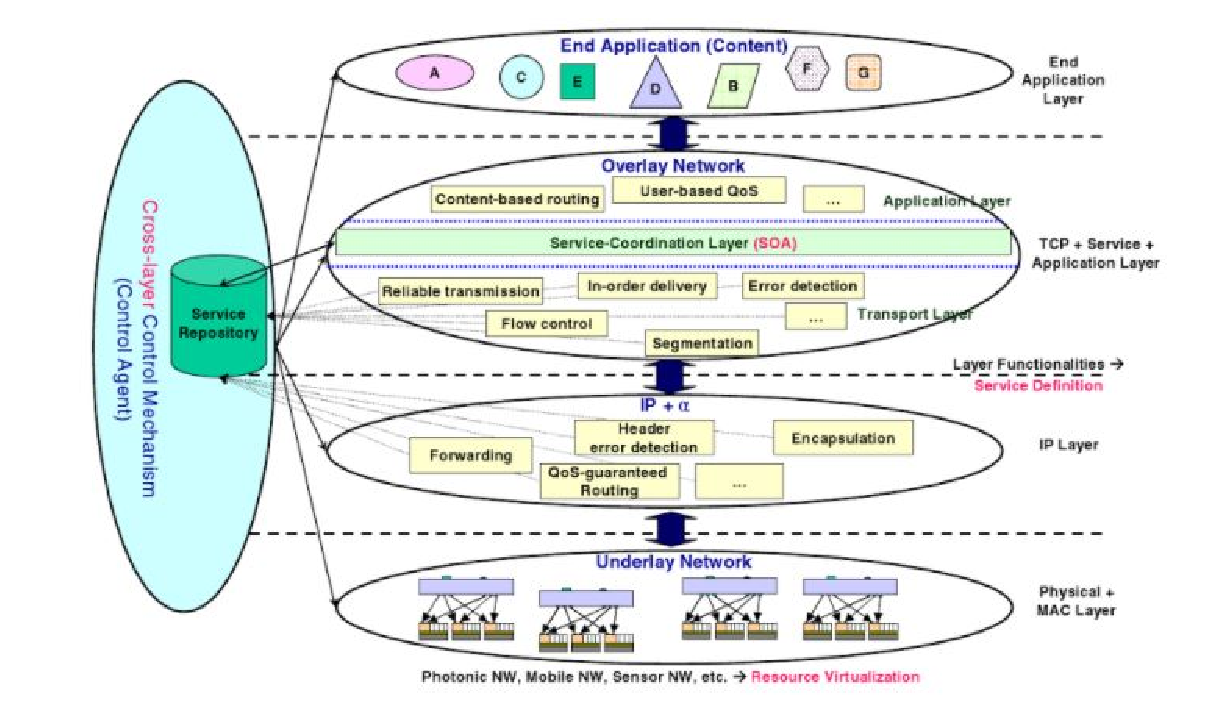
\includegraphics[width=16cm]{FCN_arc}
 	\caption{Architecture for Future Internet}
 	\label{fig: Future Network Architecture}
 \end{figure}
 The key parameters of the Future Internet are resource virtulization, cross layered architecture, service oriented architecture. The proposed architecture has four layers namely a) Physical layer (underlying physical networks) b) IP layer c) Overlay networks (virtual networks) and d) Application layer. The functionalities in each layer are implemented as services. Services are used by the service consumers requesting service providers. \newline
  
 \hspace*{0.5cm}
Network Virtualization has been considered as a long-term solution to the problem faced by the existing carrier networks \cite{1432642}. Network Virtualization creates virtualized environment that allows multiple heterogeneous virtual networks to coexist on a shared infrastructure \cite{nw_virt}. Polymorphic future Internet networks can be realized that can ensure diversification and softwarization of the networks. In network virtualization the roles of the traditional Internet service providers (ISPs) are decoupled into physical infrastructure providers (PIPs) and service providers (SPs). This decoupling results in modularization of network management. PIPs and SPs are two independent entities where PIPs owns and manage the physical infrastructure and SPs create virtual networks (VNs) by aggregating resources from multiple PIPs to offer end-to-end services. VN is the primary entity in virtualization which is a combination of active and passive network nodes interconnected through virtual links. Multiple virtual topologies can be created and deployed on a physical substrate with its both nodes and links resources are virtualized. Physical ICT (Information and Communication Technology) networks become more scalable with the deployment of coexisting multiple networks. With no changes in existing network architecture each service provider can freely implement arbitrary network with customized routing and forwarding. Conceptually, existing internet can also be considered as another VN. This helps to overcome the resistance of current carrier networks to any architectural changes.\newline
 
 The process of mapping VNs on to a physical substrate is often referred to "Virtual Network Embedding" (VNE), which deals with the allocation of virtual resources. The main challenge in embedding VNs is to how to allocate physical resources to VN elements (nodes and links) in an optimized way. This resource allocation problem is usually referred as VNE problem. Optimized allocation of resources can be based on different objectives such as different level of QoS, minimizing the cost of embedding, minimizing resource utilization, maximizing the profit by embedding more VNs and more. Many algorithms have been presented to embed VNs on a substrate infrastructure, while optimizing service-relevant metrics. These algorithms are known as VNE algorithms. Below figure (Fig. 1) illustrates the resource allocation in future Internet with the usage of network virtualization technology.\newline
 \begin{figure}[h]
 	\centering
 	\includegraphics[width=14cm, height=9cm]{vne.jpg}
 	\caption{Resource allocation in future Internet}
 	\label{fig: Network Virtualization}
 \end{figure}
 
 In the above figure SP refers to Service Providers. SPs are responsible for deploying end-to-end services. InPs refers to Infrastructure Providers who lease their physical resources to Virtual Network Providers (VNP). Virtual Network Owners (VNO) are responsible for creating, managing an operating VNs based on the requirements of SPs. Each role is independent and interacts with each other to create a VN for deploying services. VNOs uses VNE algorithms to find out suitable virtual resources that are provided by VNPs.\newline
 
 In order to increase the scalability there is a need for embedding VNs in various administrative, geographical and technical domains. This cross-domain embedding is another requirement to achieve softwarization of networks. VNs that span multiple physical networks results in coalitions and cooperation of providers which can be used to deploy multimedia services (VoIP, Online Gaming and live streaming) over multiple network domains. Such VNs can be used as a use case for Software Defined Networking (SDN) and management. An automated network management system is necessary to create and manage such virtual networks whose main functionality is to incorporate the diverse technologies, ownership and geographically different domains into an overarching single virtual network. \newline
 
 The following section briefly describes the requirements to achieve "Distributed Broker Architecture". In the thesis work, these requirements are defined and implemented to realize multi-domain orchestration and distributed brokering architecture for optimized VN Embedding. \newline
 
\subsection{Requirements}
The main requirement of the thesis is to:\newline 
 
\textit{"Deploy services across multiple operators without any knowledge of underlying topologies"} \newline
 
By creating virtual networks that span over multiple physical substrates, we can achieve scalability and better resource utilization of the underlying substrate resources. The main problem with multi-operator virtual network is none of the operators wants to disclose their topology details. In the thesis work, we introduce VN embedding algorithm that can split/distribute VNs in multiple substrates without the operators exposing their topology details.\newline
 
In order to fulfill the above requirement we derive the following sub-requirements:
 
 \begin{enumerate}					
\item \textbf{Deploying partial services on operators own domain:}
Algorithm should be capable of dividing VN request so that the divided partial VN request can be optimally embedded on to operator's own domain. The VN splitting is such that the operator maximizes the profit by leasing the resources to high revenue VN with minimum resource utilization.
\item \textbf{Communicate with peer operators for embedding partial services:}
Operators must be able to communicate with peer operators to embed partial VN, by sending/receiving messages or notifications about the VN offers. After mapping a part of VN in its own domain, operator should offer the remaining part of that VN to other operators to complete the embedding request.
\item \textbf{Orchestration:} An automated network management system to orchestrate successful embedding of virtual networks in a multi-domain substrate. The system should be able to retry a VN request excluding the pseudo node on which the first embedding failed.
\end{enumerate}	

\subsection{Outline:} 
 
This section highlights the organization of the thesis report.\newline

Chapter 2 explores state of the art techniques or related work. Existing methodologies for optimized multi-domain VN embedding and their limitations are discussed. A brief summary of related works are also provided.\newline

Chapter 3 provides an overview of the tasks carried out during the course of this master thesis. This includes lists of tasks implemented and their scope in details.\newline
 
Chapter 4 provides an overview of the proposed methodology and approaches to meet above mentioned requirements. Sub chapters include complete details on implementation phase of above mentioned requirements. This chapter also includes details of simulation set-up for carrying out experiment on proposed methodology.  Following this, the results of the experiment is documented with visual graph statistics.\newline

Chapter 5 presents future work that can be carried out as an extension to the thesis work and Chapter 6 provides a summary of the work. 

 \newpage


\section{Related Work}

Virtualization is a technique of creating virtual of something, a device, resource or an operating system. Same idea is extended to communication networks in order to make it scalable, to support diversified network services while reducing operational and capital expenditures of the network. This technique makes a network to efficiently consolidate multiple virtual structures in a single network with minimum changes to its architecture. As we mentioned in the introduction section, network sharing presents major challenges like isolation between multiple networks, their security and management. Virtualized environment to create on-demand networks, provided by network virtualization (NV) technology is considered as a possible solution to address these challenges. Heterogeneous virtual networks can be built on same physical substrate by virtualizing the resources of that physical network.  \newline

Virtual Network (VN) is the fundamental element in the network virtualization \cite{nw_virt} technology. It is the combination of virtual nodes that are connected through virtual links. Each virtual network represents network resources necessary to deploy network services such as VoIP, firewall and so on. Virtual nodes allow implementation of customized control protocols on them. In order to realize network virtualization, the virtual links connecting virtual nodes also needs to be virtualized. The users of such VNs can dynamically create, modify and remove VNs in response to the demands of the applications running on them. \newline

The participants in the network virtualization model are classified as: 1) Service Providers (SPs) and 2) Physical Infrastructure Providers (PIPs). A network service provider requests physical infrastructure provider (PIP) for resources in the form of virtual networks. The requirements of such a VN are expressed in terms of network topology, compute power, bandwidth and so on. These virtual networks can extend across multiple PIPs. Each VN is operated and managed by single SP even though the underlying PIPs are different. As a use case for Software Defined Networking (SDN) these virtual networks can be used to deploy different network services to offer customized end-to-end services to the end users. Running network functions as VNs on top of general purpose hardware can significantly reduce cost to the network operators. When using virtualization, virtual nodes and virtual links are equally important in the economic aspect. SPs are the customers in this virtualization model who buy (lease) physical resources from PIPs. But there can also be a third participant, a broker, who plays as a mediator between SPs and PIPs. A broker also manages VN request between multiple VN operators.\newline

Many research groups have presented design goals to realize network virtualization. In order to materialize network virtualization the following criteria should be fulfilled. 1) Flexibility:  Each SP should be flexible enough to deploy arbitrary VNs, customized control protocols irrespective of underlying substrate and co-existing VNs. 2) Manageability: With the separation of SPs and PIPs, network management will be modularized. Hence virtualization should provide complete control of VNs to the SPs. 3) Heterogeneity: Both VNs and underlying substrate should heterogeneous. SPs should be able to deploy cross domain end-to-end heterogeneous VNs without adhering to any specific underlying substrate technology. 4) Isolation: Coexisting VNs must be completely isolated from each other. Any misconfiguration in one VN should not affect other VNs. This improves fault tolerance, privacy and security of the VNS. 5) Scalability: Virtualized underlying networks must be able to accommodate large number of coexisting VNs without affecting their performance. 6) Legacy Support: Virtualization should support current existing Internet by treating it as another VN in the collection of other VNs.\newline

The efficient way of realizing virtualization is to create flexible inter-domain virtual networks that can span over multiple physical substrates where each substrate is separated from another not only geographically but even with different underlying technologies. Network architecture that provides end to end provisioning of virtualized resources is well described in the work \cite {arc_vn_mgmt}.

\subsection{Virtual Network Embedding}
The main challenge in mapping VNs on to the physical substrate is the optimal allocation of resources to these VNs. This resource allocation problem (VNE problem) requires algorithms that can dynamically map VNs while respecting the constraints of both VNs and underlying substrates. A VNE algorithm with dynamic resource allocation that leads to self configuring system is necessary to provide customized end to end services to end users. The optimality in the allocation of resources can be calculated with regard to different objectives that can be defined by operators, service providers or different levels of QoS. Such optimal VNE algorithm can be used to decide which virtual resources can be requested from virtual network operator.\newline

Virtual Network Embedding (VNE) algorithm deals with resource allocation of both virtual nodes and virtual links. Figure \ref{fig: VN mapping} shows two virtual networks VNR1 and VNR2 mapped on to same physical substrate. It can be noted from the figure (fig.\ref{fig: VN mapping}) that physical nodes can accommodate several virtual nodes and physical links can accommodate several virtual links. One virtual link can also span several physical links which demonstrates how several physical resources can be used to accommodate one virtual resource.


\begin{figure}[h]
	\centering
	\includegraphics[width=14cm, height=8cm]{VN.jpg}
	\caption{Virtual Networks on same substrate}
	\label{fig: VN mapping}
\end{figure}

It is well known that, resource allocation is the main part of VNE algorithms. Typically, every VN mapping comes with restrictions related to the resources. These restrictions should be obeyed by the underlying substrate. For example, if a virtual node request with compute power 'C' units is to be mapped, then the underlying physical node should have at least 'C' units of compute power. Similarly, a virtual link with bandwidth 'B' units cannot be mapped on to substrate link with bandwidth less than 'B' units. These are the basic restrictions that should be considered while embedding, but there can be other restrictions related to economy, profit, type of network services to be hosted etc. If there are more VNs, then the physical resource needs to be reserved for all VNs. This brings up the challenge of optimal resource allocation keeping in mind all the restrictions imposed by the virtual network operators.\newline

The other practical challenges for VNE are admission control for VNs. Physical substrate resources are finite and some of the incoming VN requests might get rejected or put in a queue so that resource allocation for existing VN should not be affected. Another real time issue is embedding on-line requests. It needs very less computational effort to allocate resources to a predefined set of VNs as we know the resource demand before embedding. But in real time VN requests arrive dynamically and may stay in the substrate for unknown period of time. It is very difficult to predict resource demands for on-line VNs. Embedding algorithms should be capable of serving each and every VN as they arrive, instead of serving a set of known VN requests at once. Embedding dynamic VNs are difficult because algorithm has very less knowledge about those requests. The main expectation from network virtualization is to support diverse VNs. Serving VNs with arbitrary topologies and with different technologies like different operating system, different routing mechanism might be difficult.\newline

Cross-Domain Embedding: Embedding virtual networks across multiple technologies is another challenge in achieving distributed VNE. For the Future Carrier Networks to be scalable to accommodate large number of VNs and to support requirements to host diversified services with different levels of QoS, creating and hosting VNs on single physical network is not sufficient. Network operators often fragment their networks into multiple domains for administrative reasons and to cope with its management. Such fragmented domains are different from each other in terms of vendors, underlying technologies, network resource capacity and other business prospective. Existence of orchestrating system to create and monitor VNs deployed on such heterogeneous physical domains is more important. Such a system should be able to interact with different technical domains in order to create, manage and monitor VNs that are embedded on top of these domains. The main question that arises from an orchestrating entity is- where to embed which part of VN in which technical domain so as to meet the embedding objectives. Several heuristic and exact solutions \cite{vne_survey} have been proposed on how to configure a system that can simultaneously embed large number of VNs and solve the optimal resource allocation problem.\newline 

The main challenge with multi-domain embedding is that, underlying PIPs may want to hide their topology details from their competitors. In such a situation, it is very difficult for an orchestration system to know about complete topology information of these domains. In most of the recent solutions to the multi-domain embedding, orchestrating entity assumes the knowledge of physical domains. Earlier works on VN embedding have used two main approaches to solve VNE problem. One is through heuristic approach and other is exact solution. The following section discusses such approaches in the area of VN embedding followed by the graph models and embedding formulations used in each approach. 
\subsection{Heuristic Approaches} 
In heuristic approach \cite{h1}, mapping of virtual networks on to physical network is performed by calculating low cost physical resources that can sustain general traffic of the VNs. Resource requirements for each VN is defined in terms of a set of general traffic constraints. These traffic constraints are the assumed traffic flows between designated set of nodes, defined as a matrix. With this set of traffic constraint, set of virtual nodes and links are selected to form a virtual network such that the virtual links are capable enough to allow predefined traffic to pass through them. Then suitable physical nodes and links are selected randomly which can accommodate already created virtual networks. Out of the selected set of physical nodes and links, for each VN, a best choice of physical network is selected. \newline

In another heuristic approach \cite{h2}, author tries to embed online VNs, but limits it to a time window. Incoming VN requests are collected during a time window and then embedded on the substrate network along with the constraints posed by the VNs. A queue of VN requests is maintained and VN requests are added when they are deferred because of insufficient resource in the underlying substrate. Every VN request in the queue has its own time frame for embedding, after which the request will be dropped from the queue.  Requests with highest revenue will be picked first from the queue. Mapping virtual nodes of all VN request is performed first without embedding corresponding virtual links. For mapping virtual nodes, set of substrate nodes are selected which satisfy the constraints of the virtual nodes and then for each virtual node a single substrate node out of a set is selected which has maximum available resources.  When the substrate nodes are selected for mapping, substrate links are selected for corresponding virtual links mapping.  The k-shortest path algorithm is used to select substrate link with minimum cost between selected substrate nodes. \newline

It is inefficient to restrict virtual link to a single substrate path. Assume if a VN request with virtual link bandwidth 100 units arrives and none of the substrate link has more than 50 units of bandwidth. Such a situation requires path splitting of virtual link to accommodate on two substrate links. Link embedding algorithm with path splitting and migration is also presented in the same work \cite{h2}. \newline

The limitation of such heuristic methods is that assumptions are made regarding traffic flows in VNs and the capacity of physical substrate as infinite. Also embedding is performed on collection of offline VNs with requirements already known. In real time, VNs are dynamic and it is not possible to predict the resource demand or their traffic flows. Most of the heuristic methods \cite{h1, h2, h3, h4} uses shortest-path algorithms for edge mapping and some greedy techniques for node mapping. Without relating edge mappings to node mappings, algorithm restricts the solution space, and may result in poor performance. Also the approaches explained here presents method for mappings of VNs only in one single physical domain. Cross-domain embedding is not possible with such assumptions and smaller substrate size. \newline


\subsection{Integer Linear Programming Approach} 
write about ILP, MCF, MIP

\subsubsection{Co-ordinated Node and Link Mapping:}

All the previous heuristic approaches presents VN embedding methods with clear separation of node mapping and link mapping. Embedding process is carried out in two phases by embedding virtual nodes in first phase and then embedding virtual links in another phase. Embedding VNs without any relation between node mapping and edge mapping will restrict the solution space for VNE problem and may result in poor performance of the algorithm.  \newline

A coordinated node and link mapping is presented in the work \cite{coord_map} by formulating VNE problem as Mixed Integer Programming (MIP). This work provides the basics for next set of VNE algorithms that are more effective in mapping VNs on to physical substrate. MIP problem contains decision variables of an objective function. These variables are constrained to be integer values and are used to model yes or no decisions. The objective of such a problem is a linear function that can be minimized or maximized. Such kind of objective functions with constraints is useful in solving optimization problems like optimal resource allocation. \newline

In coordinated node and link mapping \cite{coord_map} a better correlation between node mappings and link mappings is introduced. Two VNE algorithms 1) Deterministic Virtual Network Embedding (D-ViNE) and 2) Randomized Virtual Network Embedding (R-ViNE) are presented. These algorithms allow mapping of virtual links to physical links right after the mapping of virtual nodes is performed. Since solving MIP is known to be NP- hard, using MIP for optimal VN mapping is also NP-hard. So the integer program is made as linear programming formulation.  After that above mentioned algorithms D-ViNE and R-ViNE are used in linear programming solution to approximate the values of binary variables in original MIP. Then mapping of virtual nodes and virtual links is performed. This work tries to address the limitations of heuristic approach such as a) embedding offline VNs b) ignoring node or link requirement c) assuming substrate capacity as infinite and d) assuming all VN topology similar.  This method focuses mainly on embedding online VNs using MIP formulations.\newline

\begin{figure}[h]
	\centering
	\includegraphics[width=14cm, height=8cm]{coord_map.jpg}
	\caption{Substrate and VN}
	\label{fig: substrate and VN}
\end{figure}


Network Model: 
Substrate network and virtual network is modeled as weighted graph G= (V, E) where V is set of vertices ad E is set of edges connecting the nodes. Substrate network is denoted by $(G^{S}= N^{s}, E^{S})$, where 'S' denotes substrate. Each substrate node $n^{s} \epsilon N^{S}$ has CPU capacity $c{n^{s}}$ along with its location details $loc(n^{s})$. Physical link between two substrate nodes i and j (i,j $\epsilon N^{S}$) is represented by $e^{s}(i, j) \epsilon E^{S}$ with bandwidth $b(e^{s})$. Similarly virtual node is denoted by $G^{V} = (N^{V}, E^{V})$. Each VN request is associated with distance variable $D^{V} \ge 1$ which represents maximum distance from the location specified $loc(n^{v})$ by a virtual node $n^{v} \epsilon N^{V}$. Available CPU resource at substrate node $n^{s}$ is given by $R_{N} n^{s}$ which is the result of remaining CPU resource at that substrate node after assigning it to one of the virtual node. Similar variable is defined for physical link's bandwidth resource that is $R_{E}(e^{s})$ where E is substrate edge and e is virtual edge. Fig. 4 shows a substrate network and a VN request, where the numbers on the links(lines) represent available bandwidth and the numbers in rectangles(nodes) represent available CPU resources.\newline

VN Embedding process is divided into two major components node assignment and link assignment. When a VN request arrives, mapping takes place in two steps: \newline

1. Node Assignment: Virtual nodes of a VN are mapped to those physical nodes which have sufficient CPU resource to satisfy virtual node's CPU demand. Also the distance between two substrate nodes, on which virtual nodes are mapped, must be less than or equal to $D^{V}$. Formulation for node assignment is given by:

\begin{equation}
M_{N}: N^{V} \rightarrow N^{S}
\end{equation}
where $M_{N}$ represents mapping of $N^{th}$ node, $N^{V}$ represents  $N^{th}$ virtual node and $N^{S}$ represents  $N^{th}$ substrate node.\newline

Subject to 
\begin{equation}
\begin{split}
c(n^{v})  \;\leq \; R_{N}(M_{N}(n^{v})) \\
dis(loc(n^{v}) , \;loc(M_{N}(n^{v})) ) \; \leq\; D^{V}
\end{split}
\end{equation}
where $c(n^{v})$ is the capacity demand from virtual node $n^{v}$, \;$R_{N}(M_{N}(n^{v}))$ is the available resource of substrate node 'N', if it is mapped with virtual node $n^{v}$. dis(i, j) denotes distance between two substrate nodes i and j.\newline
2. Link Assignment: Each virtual link $e^{v} \;\epsilon \;E^{V}$ is mapped on to the substrate link connecting the substrate nodes on which the end nodes of this virtual link is mapped. Formulation for link mapping is given by:\newline

\begin{equation}
M_{E}: E^{V} \;\rightarrow \;P^{S}
\end{equation}
where $M_{E}$ represents edge mapping, and $P^{S}$ is set of all the substrate links.\newline

Subject to 
\begin{equation}
b(e^{v})  \; \leq \; R_{E}(P) \;\forall P \;\epsilon \;M_{E}(e^{v})
\end{equation}
As we mentioned earlier, objective functions can be maximized (minimized) depending upon the optimality factor. If suppose a netwrok operator wants to increase its revenue by mapping more number of VNs , then the VNE problem can be modeled as a optimization problem whose objective is to maximize revenue. So the goal function can be defined as maximizing the number of VN mappings by minimizing physical resource utilization. The basic VN resource constraints (eqn. 2 and eqn. 4) is still applied along with goal function. The formulations provided in this work is the basis for future embedding algorithms that we are going to discuss in next set of approaches. The set of integer constraints presented in \cite{coord_map} are computationally intractable. Those constraints are relaxed to obtain linear program and the solution is applied to D-ViNE and E-ViNE techniques. D-ViNE accepts online VN requests and maps them on to substrate one at a time. Mapping decision is solely based on previous VN requests. The linearized solution of MIP used in this technique will help in breaking the ties in selecting unmapped substrate node. After successful mapping of nodes, multi-commodity flow algorithm is used to map virtual links on to physical links.\newline
\hspace*{1cm}R-ViNE is similar to D-ViNE but uses randomized selection od substrate nodes instead of deterministic selection. It maintains a range of probability values for each virtual node mapped to each substrate node. Based on this probability, substrate node hosts virtual nodes of a VN request. From the experiment conducted on these two algorithms, it was observed that coordinated mapping of links and nodes results in higher acceptance ratio of VNs. The objective function presented here helps in load balancing at the substrate nodes which in turn increase VN acceptance ratio. It is to be noted that better performance and increased resource utilization is achieved compared to heuristic methods.\newline

The methods proposed above allows coordinated link and node mappings unlike heuristic methods where either node mapping or link mapping is performed using some greedy techniques. The new mathematical approach using MIP formulations is also presented for VN provisioning which increases quality of heuristic methods. This approach becomes basis for next set of MIP based VNE algorithms that try to optimally allocate resources to VNs. It is to be noted that coordination between mappings increases solution space and also increase in VN acceptance ratio. \newline

\newpage
\subsubsection{Cross-Domain Embedding} \label{CDE}
Heuristic and coordinated link and node mapping approaches introduced VN provisioning techniques using max-flow/min-cut and Integer Linear Programming methods respectively. Both approaches did not discuss on embedding VNs on multiple substrate networks and also are not optimal solutions. Embedding VNs across multiple substrates enables increased VN provisioning which in turn reduces cost of the services running on them. VNs that span over multiple substrates enables cooperation between providers and instant deployment of multimedia services. The efficient way to do this is by running multimedia services on VNs with their resources spanning multiple physical networks.\newline

Embedding VNs in single substrate is often non-realistic in today's world of increased number of internet users and its services. Embedding across multiple domains are more practical because, for one substrate it is almost impossible to manage an entire virtual network end-to-end. Inter-domain (cross-domain) embedding provides the service providers, a low cost end-to-end services which in turn decreases the cost of  internet services to the end users. Different internet services have different requirements like data transmission across geographically separated networks. Such services require VNs across multiple domains. But inter-domain embedding comes with the cost of knowing topology information of all the underlying domains which is another challenge addressed in the recent research .\newline

Mapping VNs over multiple physical substrates arises one important question. That is, how to split VN request over the substrates while reducing the cost for infrastructure providers (Infps). Author in \cite{vn_multiple} introduces algorithm, which is first of its kind, for mapping VNs over multiple substrates. Splitting VNs is solved using both heuristic and Linear programming method. Also algorithm to simultaneously map virtual links and virtual nodes is presented. VNE problem is formulated by considering the participants: infrastructure provider (Infp) and VN provider. Mapping VNs over multiple physical substrates is performed in three steps, 1) Resource matching 2) Embedding and 3) Binding. Infp must publish its resource details to VN providers and when a VN provider receives VN request, identify suitable substrates based on the resource information exposed by every Infp. VN provider must split the VN request to match against each Infp at a high level of abstraction. Each single Infp will embed the virtual node and virtual link on the appropriate substrate node and substrate link identified in matching phase. The following section explains the three steps (matching, embedding, binding) in details.\newline

Both substrate and VN request is modelled as a weighted graph G = (V, E) where 'V' is set of nodes and 'E' is set of links connecting those nodes. Substrate network is represented by a graph $G^{S} = (N^{S}, L^{S})$ where 'S' denotes substrate, VN request is represented by a graph $G^{V} = (N^{V}, L^{V})$ where 'V' represents virtual network. A substrate $G^{S}$ belonging to a particular Infp is denoted by $G^{S}_{Infp}$.\newline

1. Resource Matching: VN provider performs resource matching phase based on each VN request resource descriptions and Infp resource descriptions. Every node whether its a virtual node or a substrate node includes details of links attached to it. So, resource matching is only performed between nodes of VN request and physical substrate. 	In this phase a set of substrate nodes $Match(n^{v})$ capable of hosting a virtual node $n^{v} \epsilon N^{V}$ is derived. For every VN request that arrives at VN provider, $Match(n^{v})$ is calculated such that $Match(n^{v}) = {n^{s}} \epsilon G^{S}_{Infp}$.\newline

\begin{figure}[h]
	\centering
	\includegraphics[width=10cm, height=6cm]{vn_splitting.jpg}
	\caption{Splitting of VN request}
	\label{fig: VN splitting}
\end{figure}


2. VN Request splitting: For every virtual node, VN provider finds out several substrate nodes in multiple Infps from the above resource matching step. Now that for each virtual node there are several Infps, VN provider has to decide which virtual node should be embedded in which Infp. After deciding the Infp, VN provider will split the VN request to compose sub-requests that can be embedded into target Infp. The main problem here for the VN provider is to find an optimal way of splitting VN request over the Infps. For this optimal problem 'cost' of each Infp is considered. The 'cost' refers to VN provisioning cost, that is the total cost of all the resources used to embed a VN. Each Infp has its own cost for lending its resources for virtual networks. In order to solve this optimal problem, both heuristic ad exact solution based techniques are proposed. Exact based solution technique uses formulations in the form of quadratic program. Figure (fig. 5) shows an example of how VN splitting happens between two Infps $Infp^{\alpha}$ and $Infp^{\beta}$ where i, j ,k are virtual nodes and $C_{i}^{\alpha}, C_{j}^{\alpha}$ and $C_{i}^{\beta}, C_{j}^{\beta}$ are the cost for embedding the virtual nodes i, j in the infrastructure $Infp^{\alpha}$ and $Infp^{\beta}$ respectively.\newline

3. VN Embedding: From the VN splitting step, VN provider finds a optimal Infp for each virtual node which should host the sub VN request designed to it. In this step, for virtual node and virtual link of the sub VN request a suitable substrate node and substrate path is selected to ensure optimal embedding. Author proposes an exact solution method to simultaneously embed virtual nodes and virtual links of a VN request in an optimal way. Figure (fig. 6) shows embedding step for split VN graphs $G'_{v}$ and $G''_{v}$.

\begin{figure}[h]
	\centering
	\includegraphics[width=6cm, height=6cm]{vn_embedding.jpg}
	\caption{Embedding of sub VN requests}
	\label{fig: VN embedding}
\end{figure}

With the experiment on VN splitting algorithm, it was noted that exact solution based method is faster than the heuristic method to find an exact optimal solution. The objective of this work was to present an exact embedding algorithm that can simultaneously perform optimal node and link mapping in one phase. The proposed method is the first to embed online VNs that arrive in dynamic and unpredictable time. Apart from heuristic and exact methods, the work also presents MIP formulation for VN embedding. The objective function of a linear program presented here aims at minimizing the VN embedding cost. Objective function and constraints presented in this work is shown below.

\newpage
\subsubsection{Efficient Inter-Domain Embedding} \label{inter-domain}
Inter-domain embedding algorithms require more information about the substrates participating in the embedding process. The algorithms designed for intra-domain embedding does not work with inter-domain embedding. In a single domain embedding the infrastructure providers (Infp) has complete knowledge of the substrate topology and obvious knowledge about the VN request. Thus, it is very much easy that the Infp can straight away make optimal embedding calculation according to the objectives predefined. But for inter-domain embedding, Inps does not know each others topology details. So service provider has to co-ordinate with every Infp who are willing to participate and then a decision is made about mapping individual VN components to the suitable Infp. This is a major drawback when a service provider wants to deploy very large VN in less amount time. Hence a third party broker is essential to decouple service provider and Infp for a flexible and robust inter-domain VN embedding.  T\newline

In the previous section (section \ref{CDE}) we discussed cross domain embedding approach that uses integer linear programming method for solving optimal allocation problem. Here in this section, we discuss another cross-domain embedding approach which presents information sharing scheme between the Inps as most of the Inps are reluctant to expose their topology details. We earlier understood the new roles in the network virtualization technique. Same basic roles (service provider-SP and Infps) are extended in the work \cite{6914301} by adding a broker like role called as virtual network provider (VNP) in order to make centralized embedding decisions. The information sharing scheme presented here allows VNP to have partial knowledge of underlying substrate topologies. \newline

Most of the previous algorithms perform embedding set of collected VN requests i.e. offline requests. An algorithm to embed online VN requets is developed by  estimating intra-domain topologies with an augmented network. This helps in coordinating node and link mapping. Decomposing VN requests into sub-VN requests based on augmented topology and introduction of integer linear programming formulation results in embedding online VN requets in polynomial time. Here we introduce the main concepts presented in the work \cite{6914301} to support inter-domain embedding along with ILP formulation.

\begin{enumerate}[label=(\Alph*)]
\item Business Roles: 

\begin{enumerate}
\item Service Provider (SP): Service Providers are the customers for virtual network providers (VNP) and request virtual network topology to run on Infps. SP requests VNP with specific resource requirements which is used to create a virtual topology. SPs run their services on top of these VN to provide value based services to the end users.

\item Virtual Network Provider (VNP): VNPs are broker like agents who mediate between SPs and Infps. VNP receives VN request from SP and decompose it into the components like virtual nodes and virtual links. Then these components are embedded on the physical substrates with the help of inter-domain embedding algorithm. 

\item Infrastructure Providers(Infps): These are the operators who lease their physical network resources to deploy virtual topologies. Each Infps provide resources requested from VNP according the agreement between them.
\end{enumerate}	
In this work VNP is assumed to be unique which can communicate with every participating Infps. Any VN request involves SP who does not care about physical substrate or the embedding technique, except requesting VNP with VN requirements and paying for it. Similarly underlying physical substrate does not bother about VNs running on them except serving the resource request made by VNP. By this way SPs and Infps are decoupled with the introduction of VNPs.
	
\item Information Sharing Scheme:

The solution presented here prevents service providers from multiple negotiations with every Infp and also protects each Infps private information. The new role in the system VNP communicates and negotiates with Infps on behalf of SPs. For this, VNP decomposes a VN request and embeds on the physical substrate. In general the cost of embedding in intra-domain links is cheaper than that of external links. so a VNP, in order to maximize its profit and to minimize the expenditure tries to embed maximum parts of a VN request in the same substrate. This requires each Infp to expose partial information about their resource capacity to the VNPs. 

A VN request comes with resource requirements and desired locations, that is in which physical substrate a particular virtual node has to be embedded. Along with these attributes, each virtual node has a restriction which represents the maximum distance from which the node can be embedded from its desired location. So the resource demand by each virtual node of a VN request is represented by a triple <required capacity, desired location, distance constraint>. An example of a simple VN request is pictured in the figure .\ref{IDE_VN} (a) where, the numbers on the links represent required bandwidth demand of the corresponding virtual link. The figure .\ref{IDE_VN} represents the information known to each role SP, VNP and Infp.
\begin{figure}[h]
	\centering
	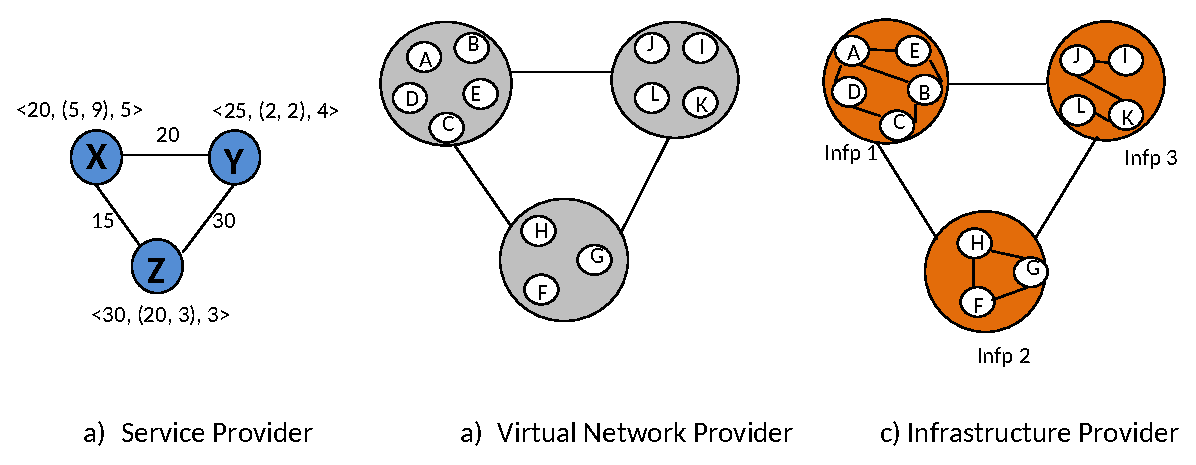
\includegraphics[width=\linewidth]{inter-domain}
	\caption{Level of Information known to each Role}
	\label{IDE_VN}
\end{figure}

A service provider only knows what resource requirements it needs for the VN topology. The information about underlying substrate is not known to the SP. Similarly VNP only knows which Infps are participating or ready to lease their physical resources. And Infps have knowledge of their own topologies only. 
Since for VNPs, physical substrate information is critical and Infps does not want to expose it, the information sharing scheme allows Inps to provide a) node location, node capacity and price b) vertices, available bandwidth and unit price of inter-domain link c) length-based price intra-domain links. From this set of information. VNP can easily allocate resource by minimizing the cost in a optimal way since it now has the knowledge of resource price and resource capacity. 

\item 	Inter-Domain VN Embedding:

With the help of business model presented (fig .\ref{IDE_VN}) and the information sharing scheme the embedding process can be carried out in the following steps:

Step 1:  VN Request decomposition: After receiving VN request from the SP, VNP starts decomposing (fig .\ref{IDE_decomp}) the VN into multiple components in a best way, such that the decomposition minimizes the overall expenditure/cost. The next step is to pre-locate the virtual nodes in the substrates. For pre-locating virtual nodes, a set of candidate substrate nodes are selected who can support the resource demands of each virtual node. In the example candidate set for virtual node 'X' is \{A, B\}, 'y' is \{C, D\} and 'Z' is \{J\}.  Locating virtual nodes in this stage also affect path selection for virtual links. Therefore the cost of embedding nodes and links depends on each other. And for VNP, the substrate topology is invisible which makes path selection for virtual link difficult. To overcome this, author assumes a mesh topology for every participating substrates. 

\begin{figure}[h]
	\centering
	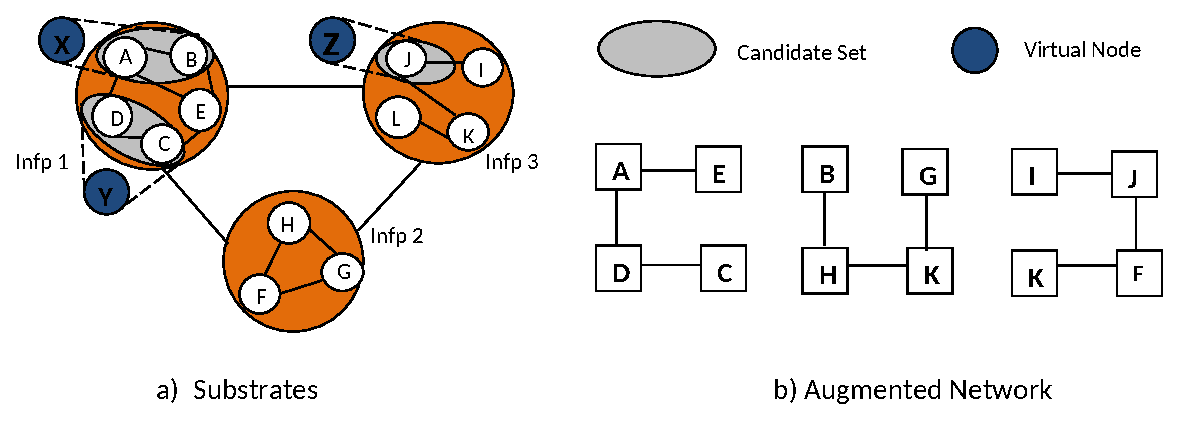
\includegraphics[width=\linewidth]{inter-doamin_1}
	\caption{VN Decomposition}
	\label{IDE_decomp}
\end{figure}
An augmented network (see fig .\ref{IDE_decomp})is derived by estimating intra-domain topologies which helps VNP to coordinate node mapping and link mapping while decomposing VN request. Because of the co-existing node and link constraints, the embedding problem becomes NP-hard and hence formulation is requires for the optimal embedding. Decomposed VN request is then sent to the Infps for the actual embedding.

Step 2: Sub-VN request processing: Each participating Infps receive their own share of decomposed VN request from the VNP. These sub-VN requests are embedded by Infps in their own domains based on their own strategies. This phase has same existing intra-domain embedding procedure. From the step 1, virtual nodes of sub-VN requests are already embedded on to the substrate nodes. So the only task for Infps is to map corresponding virtual links from the sub-VN requests. Each Infp will respond to the VNP with either success message or failure message indicating the embedding result of their portion of VN request. 

Step 3: Substrate Resource Allocation: If VNP receives success message from all the Infps, then embedding is considered as success for that particular VN request. For successful embedding VNP replies every Infp with confirmation message to continue with the actual resource allocation to the sub-VN requests. If even one failure message is received from the Infps then the embedding of whole VN request is considered as failure and VNP proceeds to next VN request terminating the current one.

\item Formulation for Embedding:  
 
 Each substrate and VN are modelled as undirected graph $G^{S} = (N^{S}, L^{S})$ and $G^{V} = (N^{V}, L^{V})$ respectively, where $N^{S}$ is set of substrate nodes, $L^{S}$ is set of substrate links and $N^{V}$ is set of virtual nodes, $L^{V}$ is set of virtual links. Each substrate node $n^{S} \epsilon \; N^{S}$ is associated with its geographic location $g(n^{S})$, its available CPU capacity $C(n^{S})$ and a domain index $dom(n^{S})$ representing the domain it belongs. Each substrate link $l^{S}(u, v) \epsilon \; L^{S}$ between the pair of nodes (u, v) has bandwidth capacity $B(l^{S})$. 
 Let  $p^{S}(m^{S}, n^{S})$ be the set of all possible path from source node $m^{S}$ and destination node $n^{S}$. The available bandwidth of the path $p^{S}$ is given by 
 \begin{equation}
 R(P^{S}) = \min_{l^{S}\epsilon p^{S}}B(l^{S})
  \end{equation} 
Similar to the substrate node, each virtual node $n^{V} \epsilon \; N^{V}$ is associated with its desired location $g(n^{V})$, its CPU demand $C(n^{V})$ and non-negative radius $d^{V}$ representing distance constraint. The capacity demand of each virtual link $l^{V}\epsilon L^{V}$ is denoted by $B(l^{V})$. A candidate set for the virtual node $n^{V} \epsilon N^{S}$ is given by $\theta(n^{V})$ which is a set of all possible substrate nodes that satisfy the distance constraint of the virtual node $n^{V}$. Hence 
\begin{equation}
\theta(n^{V}) = \{n^{V} \epsilon N^{S} | dis(g(n^{V}), g(n^{S})) \leq d^{V}\}
\end{equation}
Augmented network is given by $G^{A} = (N^{A}, L^{A})$ where $N^{A} = N^{S} \cup N^{V}$ and $L^{A} = L_{vs} \cup L^{ss}$. $L_{vs}$ is a set of inter-domain links and $L^{ss}$ is a set of intra-domain links. Augmented path set is given by $p^{A}(m^{A}, n^{A})$ and available bandwidth for the augmented path set is given by 
\begin{equation}
R(P^{A}) = \min_{l^{A}\epsilon p^{A}}B(l^{A})
\end{equation} 

When a VN request $G^{V}$ arrives at VNP, it pre-locates $G^{V}$ in the augmented network $G^{A}$ for which the VN is decomposed into multiple sub-VN requests. After that each Infp will be assigned with this sub-VN request. So the first phase of VN assignment starts with VNP mapping nodes and links onto the augmented network. Even though the substrate nodes are capable of hosting multiple virtual nodes, only one virtual node per VN request is mapped to one substrate node at a time. Hence node mapping $M_{N} : N^{V} \rightarrow N^{A}\;  \forall n^{V}, m^{V} \epsilon N^{V}$ from virtual nodes to augmented nodes is given by: \newline
s
\hspace*{5cm}$M_{N}(n^{V}) \epsilon \;\theta(n^{V})$

\hspace*{5cm}$M_{N}(m^{V}) = M_{N}(n^{V}) \text{, iff } m^{V}=n^{V}$

\hspace*{4cm}subject to 

\hspace*{6cm}$C(n^{V})  \leq C(M_{N}(n^{V}))$ \newline

Similarly link mapping for every virtual link is given by: \newline 

\hspace*{5cm} $M_{L} : L^{V} \rightarrow P^{A}$ such that

\hspace*{5cm} $M_{L}(m^{V}, n^{V}) \subseteq P^{A}(M_{N}(m^{V}), M_{N}(n^{V}))$

\hspace*{4cm} subject to
 
\hspace*{5cm} $B(l^{V}) \leq R(P^{A})$ \newline

After decomposing VN request each sub-VN request is assigned to every domain i, denoted by $G^{\overline{V}}_{i} = (N^{\overline{V}}_{i}, L^{\overline{V}}_{i})$. VNP has already decided the mapping of each node $n^{\overline{V}} \epsilon \; N^{\overline{V}}_{i}$ on to the substrate node belonging to the domain i. So, the only task for an Infp which owns the domain i is to select the substrate node $n^{S}$ for each $n^{\overline{V}}$ such that \newline


\hspace*{5cm}$M_{\overline{N}}(n^{\overline{V}}) = n^{S}$

\hspace*{4cm}subject to 

\hspace*{6cm}$dom(n^{S}) = i \text{ and } g(n^{S}) = g(n^{\overline{V}})$  \newline

The link mapping inside every Infp finds a set of substrate paths and is denoted by $M_{\overline{L}} : L_{i}^{\overline{V}} \rightarrow P^{S}$ such that

\hspace*{5cm} $M_{\overline{L}}(m^{\overline{V}}, n^{\overline{V}}) \subseteq P^{S}(M_{\overline{N}}(m^{\overline{V}}), M_{\overline{N}}(n^{\overline{V}}))$ \newline

\hspace*{4cm} subject to

\hspace*{5cm} $B(l^{\overline{V}}) \leq \sum_{P^{S}\epsilon M_{\overline{L}}(l^{\overline{V}})} R(P^{S})$ \newline

Embedding of VN request is considered success only if VNP mapping and Infp mapping are successful. Otherwise the embedding for that VN request is considered as failure.
\end{enumerate}

We have now methods for VNP assignment and Infp assignment and these two process are the two key problems in embedding VN requests. Here we present objective for VNP and Infp in order to optimally allocate resources to each VN request. Every Infp have their own cost for leasing their resources to the sub-VN requests denoted by c(.). Hence for a sub-VN request $G^{\overline{V}}_{i}$ assigned to the Infp 'i', the cost of embedding is denoted by $C^{-}(G^{\overline{V}}_{i})$ which is the sum of the product of the amount of resource allocated and the cost for using that resource. Since VNP is charged by Inps for corresponding sub-VN requests, the final cost for embedding a VN request is equal to the total revenues of Inps for embedding all the sub-VN request of that VN. Hence the objective of the VNP assignment is to minimize the total cost of embedding while decomposing a VN request and respecting the capacity constraints. Since node mapping is done in the VNP assignment phase, each Infp tries to minimize the cost of link embedding while mapping sub-VN requests. If each virtual link is considered as a commodity flow in the augmented network $G^{A}$, then VNP assignment is considered as multi-commodity flow problem (MCF). For large number of substrate topologies, traditional techniques for solving MCF is computationally intractable, integer linear programming (ILP) is necessary to formulate embedding. ILP formulation is presented for both VNP and Infp assignment with same set of objectives for both. \newline

In this work, virtual links are assumed to be unsplittable in link mapping phase. And also for node mapping best-fit and first fit heuristic methods are used. In best-fit, candidate substrates with lower costs are used and in first-fit available first substrate nodes are used. For simulation, 4 domains each with 30 nodes and 72 links are created. Virtual networks are also generated with number of nodes randomly determined by uniform distribution between 5 and 10. The probability of two nodes connected by a link is 0.4 and capacity requirements of each node is  randomly determined by uniform distribution between 0 and 20.  Comparing the proposed method with best-fit, the proposed method achieves higher acceptance ratios and lower resource utilizations simultaneously. Best-Fit algorithms follows greedy method for mapping nodes which might result in longer substrate paths to support virtual links. 

In order to increase the VN acceptance ratio, author proposes 'deadline-based scheduling' where a failed request is put into queue with a time deadline instead of rejecting it. Whenever a VN is nearer to its deadline it is given a higher priority for the next embedding attempt. This scheduling method can be modified to maximize the profit by scheduling failed VN requests based on their revenue. VN requests with higher revenues are given high priority for next round of embedding. These two methods affect each other because VN requests with larger resource demands are satisfied in less time resulting in failure of requests with smaller resource demands. This in turn decreases acceptance ratio. A balance needs to be made between making more revenue and embedding more VNs. \newline

\hspace*{1cm} An efficient solution for inter-domain embedding is presented in this work. A new information sharing scheme is also presented with an additional role of VN provider. By estimating the substrate topologies heuristic algorithm is proposed to embed online requests in a polynomial time. Even though ILP formulation is presented for decomposing the VN request in the VNP phase, actual node mapping inside a substrate is performed by heuristic approaches like best fit and first-fit. Estimations are made regrading the topologies of Infps and it is assumed that all the participating Infps are ready to expose partial information about their domains.  





\subsubsection{Edge Wise Node Mapping (EdWiN)} \label{edwin}

All the previous algorithms presented VN embedding methods based on heuristic and exact solution approaches for separate, coordinated and simultaneous mapping of virtual nodes and virtual links. As we know VN embedding is a resource allocation problem. Such an problem is characterized by large number of solutions and finding a best solution depends on some aim or overall objective that is implied in the problem statement. The best optimal solution is that solution which satisfies the condition of the problem as well as the objective of the problem. \newline
Many previous works presented an optimal VN embedding solutions using Mixed Integer Programming (MIP) formulations. MIP is a mathematical optimization program in which the some or all of the variables are integers. MIP is used in linear programming in which an objective function and constraints related to it are present. The objective function is the goal of the linear programming which can either be maximized and/or minimized and constraints represents restrictions of the problem.

The methods presented in the work \cite{vn_multiple} is the first step in mapping VNs in multiple domains. It also provided a model to simultaneously map multiple VN requests using lookahead property. Another linear programming based VN embedding approach is presented in the paper \cite{vneapproach}. The method proposed here aims at embedding VNs with larger lookahead values with predefined policies. New set of MIP formulation is presented for supporting larger lookahead values and the formulation is named as EdWiN: Edge Wise Node Mapping. Also new approach for describing both substrate structure and virtual networks is provided. The flexibility in describing the physical substrate and virtual networks in this work leads to many use cases for management and orchestration of Software Defined Networks (SDN). SDN decouples control plane and data plane which allows running network applications on top of virtual machines connected to controllers in the control plane. EdWiN method can be used in modelling virtual machines as virtual nodes and using virtual links to connect them. This approach of virtualization can be used as the basic component in the management and orchestration of future carrier networks. Figure \ref{fig: Network Orchestration} shows reference architecture of network orchestration where the network
orchestrator receives VN requests from VN owners and are embedded into virtualised infrastructures.\newline

\begin{figure}[h]
	\centering
	\includegraphics[width=14cm, height=4cm]{sdn_orc.jpg}
	\caption{Network Orchestration}
	\label{fig: Network Orchestration}
\end{figure}


The formulation presented here is the basis for the formulations presented in the thesis work. Substrate model and VN model is also used in the thesis work. The network orchestrator concept presented here is also taken for the thesis work to design distributed broker architecture. The main functionality of the orchestrator is to dynamically dispatch virtualized resources to network functions. The following section provides the basic graph model and formulation used for simultaneous, optimal embedding of multiple VNs. 

\begin{enumerate}[label=(\Alph*)]
	\item  Substrate model: \label{sub_model}
	
	Both physical and virtual networks are modelled as undirected graph \textit{G=(V, E)} where \textit{V} is the set of vertices and \textit{E} is the set of edges. 
	The model for physical substrate \textit{$G^{S}= (V^{S}, E^{S})$} is characterized by 
	\begin{itemize}
		\item A set of  \textit{N} nodes \textit{$V^{S}=\{n_{1}, n_{2}...n_{N}\}$}
		\item A set of \textit{$L \leq$ N(N -1)} edges \textit{$E^{S}=\{e_{ij}\}_{i,j \epsilon \{1...N\}, ;\ i \ne j}$} with \textit{$e_{ij}\equiv e_{ji}$}
		\item  Node capacity matrices, for example:\newline
		- CPU matrix $[C_{i}]_{i=1...N}$ , where $C_{i}>0 \; \forall i \epsilon \{1...N\}$ \newline
		- Memory matrix $[M_{i}]_{i=1...N}$, where $M_{i}>0 \; \forall i$ \newline
		- Storage matrix $[S_{i}]_{i=1...N}$, where $S_{i}>0 \; \forall i$ 
		\item Connectivity Matrix $B = [B_{ij}]_{i,j=1...N}$, where $B_{ii} =0$ and $B_{ij} \epsilon \{0, 1\} : B_{ij} =1$ iff $e_{ij}$ exists; $G^{P}$ is an undirected graph, thus $B_{ij} = B_{ji}$
		\item Link capacity matrix $B_{c} = [B_{c_{ij}}]_{i,j=1...N}$, where $B_{c_{ii}} = 0$ and $B_{c_{ij}} \geq 0 \; \forall i,j\;\epsilon \;\{1...N\}; \;e_{ij}$ has capacity $B_{c_{ij}}$; $G^{P}$ is an undirected graph, thus $B_{c_{ij}} = B_{c_{ji}}$.
	\end{itemize}
	
	\item   VN requests:  \label{vn_req}
	
	VN requests are resolved by simultaneous embedding of \textit{G} VN request, \textit{$G_{g}^{V}= (V_{g}^{V}, E_{g}^{V})$}, by splitting each VN request g $\epsilon$ \{1...G\} link wise into $g_{k}$ 2-node sub graphs. The k-th subgraph, k\;$\epsilon\{1...g_{k}\}$, of the g-th graph is characterized by: 
	\begin{itemize}
		\item Source and Destination nodes  \textit{$v_{s_{g_{k}}}$} and   \textit{$v_{d_{g_{k}}}$} with capacity requirements \textit{$C_{s_{g_{k}}}$}, \textit{$S_{s_{g_{k}}}$} and \textit{$C_{d_{g_{k}}}$}, \textit{$S_{d_{g_{k}}}$} respectively.
		\item The requested directional bandwidth \textit{$b_{g_{k}}$}
		\item  Boolean variables
		\begin{equation} \label{bl_var}
		\begin{split}
		y_{s_{g_{k}}}^{i}=
		\begin{cases}
		1, & \text{if } n_{s_{g_{k}}}\rightarrow n_{i} \\
		0, & \text{if } n_{s_{g_{k}}}\not\rightarrow n_{i} \\
		\end{cases}\\
		y_{d_{g_{k}}}^{i}=
		\begin{cases}
		1, & \text{if } n_{d_{g_{k}}}\rightarrow n_{i} \\
		0, & \text{if } n_{d_{g_{k}}} \not\rightarrow n_{i} \\
		\end{cases}
		\end{split}
		\end{equation}
		where a $\rightarrow$ b implies \textit{a} is embedded in \textit{b} in the solution.
		
		\item Boolean variables $x_{ij}^{g_{k}}$, with value 1 if \textit{k -th} subgraph of the \textit{g-th} request uses bandwidth on the physical link $e_{ij}$. Hence, 
		\begin{equation}
		x_{ij}^{g_{k}} \epsilon \{0, 1\} \;\forall i, j \;\epsilon\; \{1...N\}\\
		\end{equation}
		where $x_{ii}^{g_{k}} = 0, \; \forall i \;\epsilon\; \{1...N\}$\newline
		Finally the whole VN request  $G_{g}^{V}, \; \forall g \;\epsilon\; \{1...G\}$, is characterizes by a boolean variable:
		\begin{equation} \label{bl_var1}
		y_{g}=
		\begin{cases}
		1, & \text{if }   G_{g}^{V}\rightarrow G^{P} \\
		0, & \text{if }   G_{g}^{V}\not\rightarrow G^{P} \\
		\end{cases}
		\end{equation}
	\end{itemize}
	
	\item  Cost Function: 
	
	In order to identify embedding of \textit{g}-th VN request as successful, a boolean variable $y_{g}$ is used. The cost function involves weight $w_{g}$ to characterize the priority of $y_{g}$ based on factors like price of the VN request. The second part of the cost function involves the costs that are incurred for consuming the resources to embed VN request. The variable $w_{e_{ij}}$ represents cost for using resource on the physical link $e_{ij}$. The variables $w_{C_{i}}$, $w_{M_{i}}$ and $w_{S_{i}}$ represents costs for using compute, memory and storage resources at physical substrate node i. With these variables the goal function is modelled as:
	\begin{equation} \label{edwin_gf}
	\begin{aligned}
	max \big\{ \sum^{G}_{g=1}\big[ w_{g} y_{g} &- \sum^{K_{g}}_{k=1} \sum^{N}_{i=1} \sum^{N}_{j=1} w_{e_{ij}} b_{gk} x^{gk}_{ij}\\ &- \sum^{K_{g}}_{k=1} \sum^{N}_{i=1} \big(w_{C_{i}} \big( C_{s_{g_{k}}} y^{i}_{s_{g_{k}}} + C_{d_{g_{k}}} y^{i}_{d_{g_{k}}} \big) + w_{M_{i}} \big( M_{s_{g_{k}}} y^{i}_{s_{g_{k}}} + M_{d_{g_{k}}} y^{i}_{d_{g_{k}}} \big) + w_{S_{i}} \big( S_{s_{g_{k}}} y^{i}_{s_{g_{k}}} + S_{d_{g_{k}}} y^{i}_{d_{g_{k}}}\big) \big)\big]\big\}
	\end{aligned}
	\end{equation} 
	
	The above goal function (objective) provides optimal solution for resource allocation by maximizing the profit by embedding more VNs with high revenue while minimizing resorce utilization at the substrate nodes and substrate links. The first term is to maximize VN embedding, second term is for minimizing the bandwidth utilization and third term is for minimizing the utilization of compute, memory and storage resources at the physical substrate. \newline
	
	\item  Constraints: 
	\begin{enumerate}
		\item  Topology Constraints: The link \textit{$e_{ij} \; \forall i, j \epsilon \{1...N\}$} can be used only if that link exists:
		\begin{equation}
		\begin{aligned}
		x^{gk}_{ij} \leq B_{ij}, \forall g \epsilon\{1...G\}, \forall k \epsilon\{1...K{g}\}
		\end{aligned}
		\end{equation} 
		
		\item  Capacity Constraints: For each virtual link, bandwidth allocated on each substrate link must be less than or equal to the capacity of that substrate link:
		\begin{equation}\label{edwin_cap_cons}
		\begin{aligned}
		\sum_{g=1}^{G} \sum_{k=1}^{K_{g}} \big[ b_{gk} \big( x^{gk}_{ij} + x^{gk}_{ji} \big) \big] \leq B_{c_{ij}}  \forall i, j \epsilon\{1...N\}
		\end{aligned}
		\end{equation} 
		
		For virtual nodes, the compute resource allocated must be less than or equal to the compute capacity available on the substrate node:
		
		\begin{equation}
		\begin{aligned}
		\sum_{g=1}^{G} \sum_{k=1}^{K_{g}} \big( C_{s_{gk}} y^{i}_{s_{gk}} +  C_{d_{gk}} y^{i}_{d_{gk}} \big) \leq C_{ij} \ \forall i \epsilon\{1...N\}
		\end{aligned}
		\end{equation}
Similar equations can be written for memory and storage also.
\item Embedding Constraints: 
\begin{itemize}
			\item The bandwidth flow constraints of each virtual node must be satisfied $ \forall g \epsilon \{1...G\}, ;\ \forall k \epsilon \{1...K_{g}\}$
			
			\begin{equation}\label{edwin_emb_cons}
			\begin{split}
			\sum_{j=1}^{N}  x^{gk}_{n_{j}} - \sum_{i=1}^{N} x^{gk}_{i_{n}} =  y^{n}_{s_{gk}} -  y^{n}_{d_{gk}} ;\ \forall n \epsilon\{1...N\}\\
			\sum_{j=1}^{N}  x^{gk}_{n_{j}} \leq 1, \sum_{i=1}^{N} x^{gk}_{i_{n}} \leq 1 ;\ \forall n \epsilon\{1...N\}
			\end{split}
			\end{equation} 
			
			
			\item  Source node and Destination node of each VN subgraph is embedded only once. Embedding of source and destination nodes are valid only if whole VN graph to which they belong is embedded.
			\begin{equation}
			\begin{split}
			\sum_{i=1}^{N} y^{i}_{s_{gk}} = y_{g} ;\ \forall g \epsilon \{1...G\}, ;\ \forall k \epsilon \{1...K_{g}\}\\
			\sum_{i=1}^{N} y^{i}_{d_{gk}} = y_{g} ;\ \forall g \epsilon \{1...G\}, ;\ \forall k \epsilon \{1...K_{g}\}
			\end{split}
			\end{equation} 
			
			\item Source node and destination node of the same VN is not mapped to same substrate. That is co-location of source and destination virtual nodes is not allowed.
			
			\begin{equation}
			y^{n}_{s_{gk}} +  y^{n}_{d_{gk}} \leq 1 ;\ \forall n \epsilon\{1...N\}
			\end{equation} 
			
			\item Since the VN graph is divided into sub graphs based on links, virtual node (source or destination) of one VN sub graph might be part of another VN sub graph. So $ \forall g \epsilon \{1...G\}, ;\ \forall k \epsilon \{1...K_{g}\}$		
			\begin{equation}
			\begin{split}
			y^{n}_{s_{gk}} =  y^{n}_{s_{k'g}} ;\ \forall n \epsilon \{1...N\}\quad if \quad s_{gk} = s_{k'g}\\
			y^{n}_{d_{gk}} =  y^{n}_{d_{k'g}} ;\ \forall n \epsilon \{1...N\}\quad if \quad d_{gk} = d_{k'g}\\
			y^{n}_{d_{gk}} =  y^{n}_{s_{k'g}} ;\ \forall n \epsilon \{1...N\}\quad if \quad d_{gk} = s_{k'g}
			\end{split}
			\end{equation} 
			\item Since co-location of nodes is not allowed, the separation can be forced by:
			\begin{equation}
			\begin{split}
			y^{n}_{s_{gk}} +  y^{n}_{s_{k'g}} \leq 1 ;\ \forall n \epsilon \{1...N\}\quad if \quad s_{gk} \neq s_{k'g}\\
			y^{n}_{d_{gk}} +  y^{n}_{d_{k'g}} \leq 1 ;\ \forall n \epsilon \{1...N\}\quad if \quad d_{gk} \neq d_{k'g}\\
			y^{n}_{d_{gk}} +  y^{n}_{s_{k'g}} \leq 1 ;\ \forall n \epsilon \{1...N\}\quad if \quad d_{gk} \neq s_{k'g}
			\end{split}
			\end{equation} 
		\end{itemize}
		
		
	\end{enumerate}
	
	\item  Location: 
	
	Forcing a virtual node to be mapped on to a particular substrate node might be considered as a constraint. Hence, constraint to bind a virtual node to a fixed substrate node can be given as:
	
	\begin{equation}
	\delta^{i}_{*_{gk}} 
	\begin{cases}
	1, & \text{if }   n_{*_{gk}}\rightarrow n_{i} \\
	0, & \text{ otherwise} \\
	\end{cases}
	\end{equation} 
	where * = (s, d) refers to source or destination and $a \rightarrow b$ implies node a is embedded on substrate node b. \newline
	
	Additional constraints to force fixed node embedding are $ \forall g \epsilon \{1...G\}, ;\ \forall k \epsilon \{1...K_{g}\}$ 
	\begin{equation}
	\begin{split}
	y^{i}_{s_{gk}} =  y_{g} \quad if \quad \delta^{i}_{s_{gk}}  = 1\\
	y^{i}_{d_{gk}} =  y_{g} \quad if \quad \delta^{i}_{d_{gk}}  = 1\\
	\end{split}
	\end{equation} 
	
	where i denotes a substrate node $n_{i}$ where the virtual node $n_{*_{gk}}$ must be embedded. \newline
	
	\item Variable $y_{g}$: 
	
	The variable $y_{g}$ in above equations makes it
	possible to have partial solutions of the embedding problem. $y_{g} = 1$ if VN requests can be embedded under the constraints. When none of the
	requests can be embedded $y_{g}$ becomes 0 to all for all the requests.\newline
	
	\item  Path Splitting: 
	
	Formulations presented here does not allow path splitting so a virtual link can only be embedded in one single path. But changing the variable $x^{gk}_{ij}$ from boolean to real and using Eq. \ref{edwin_cap_cons} and Eq. \ref{edwin_emb_cons} with the cost function (Eq. \ref{edwin_gf}) path splitting can be performed. 
	
\end{enumerate}

With the formulation presented here, author compares the approach with previous approaches presented as in \cite{vn_multiple}. The exact method presented in \cite{vn_multiple} simultaneously embeds multiple request which is inferred to be inefficient as it does not allow partial solutions. That is if all the VN requests are embedded then only the solution is valid. This degrades the performance of embedding. Whereas the algorithm presented in EdWiN supports partial solutions  with the help of the variable $y_{g}$. \newline

The MIP formulation presented in EdWiN is run using arbitrary topologies and each substrate node in a topology is assigned a colour with equal probability of assignment. The node capacity is same as that of the nodes used in \cite{vn_multiple}. Multiple VN requests are created with each virtual node assigned a colour. The only condition is that each virtual node must be embedded in a substrate node matching its colour. The VNs are generated sequentially and fed to the algorithm with lookahead values of 1, 20 and 40. For instance EdWin20 gathers 20 VNs and then start embedding characterized by the variable $y_{g} = 1$ by reducing the  capacity of the substrate. It is to be noted that EdWiN algorithm with 20 and 40 VNs results in higher embedding rate compared to EdWiN with 1 VN request. Convergence time might be sometimes important than the optimized embedding rate. It has been observed that the simplicity of the formulation contributes to the rapidness of EdWiN algorithm.\newline

The EdWiN algorithm presented novel MIP formulation for simultaneous embedding of VN requests with increased embedding rate. A two digit gain was observed in terms of embedding rate and resource utilization along with significant reduction in the convergence time. 
 
\subsubsection{Recursive and Hierarchical Embedding} \label{md_monitoring}

Most of the algorithms explained above perform multi-domain VN embedding by using simplified models for physical resources where underlying physical networks are modelled as flat infrastructures. In such a network scenario, each VN request is split into multiple sub-graphs. Each sub-graph is then embedded on each physical domain separately that is embedding on multi-domain and single domain separately. For instance in the work explained above in section \ref{CDE}, algorithm to split VN at broker level is based on min-cut and algorithm to embed them at domain level is based on MIP formulation.  
\begin{figure}[h]
	\centering
	\includegraphics[width=12cm, height=6cm]{nw_abst.jpg}
	\caption{Network Abstraction}
	\label{fig: nw_abst}
\end{figure}


In the paper \cite{multi-domain} author proposes the idea of 'abstracting physical networks' which makes multiple domains to appear as a pseudo flat infrastructure. This abstraction helps to reuse the previous embedding algorithms for flat infrastructure, used to embed VN at different domains separately, to apply for multiple domains. A slight modification to the existing algorithm is needed to use it for multiple domain embedding. The abstraction idea is presented in the project ETHICS \cite{EHTICS} in which each physical domain abstracts its topology in order to decide the kind of information exposed to multi domain orchestrator. In this work \cite{multi-domain} ETHICS idea of abstraction is extended to embed whole infrastructure with compute,storage and memory resources. The abstraction is done as shown in figure \ref{fig: nw_abst} where each physical domain is abstracted as a pseudo node so that a complex network with multiple domains look like a flat network. To this abstracted network we can now apply existing algorithms with modifications to suit multi domain embedding. It has been observed that embedding speed increases with level of network abstraction, that is higher the level of abstraction faster is the embedding speed, when compared to embedding with complete topology information. Also it is to be noted that, abstraction doesn't effect the performance of embedding algorithm.

In the figure \ref{fig: nw_abst} we can see each domain is abstracted into one pseudo node, for instance, domain A is abstracted into pseudo node A. The formulation presented in EdWiN (section \ref{edwin}) is modified to add more information about the resources of a physical domain. Algorithms including EdWiN does not allow multiple nodes inside single physical domain. Also embedding links on the physical nodes is important to support embedding sub graphs of a VN request into a domain. Hence, EdWiN formulation is modified to i) co-locate nodes and ii) to embed links on nodes- a) completely inside nodes and b) passing through the nodes, which also becomes main requirements for abstracting domains as nodes.\newline

\begin{figure}[h]
	\centering
	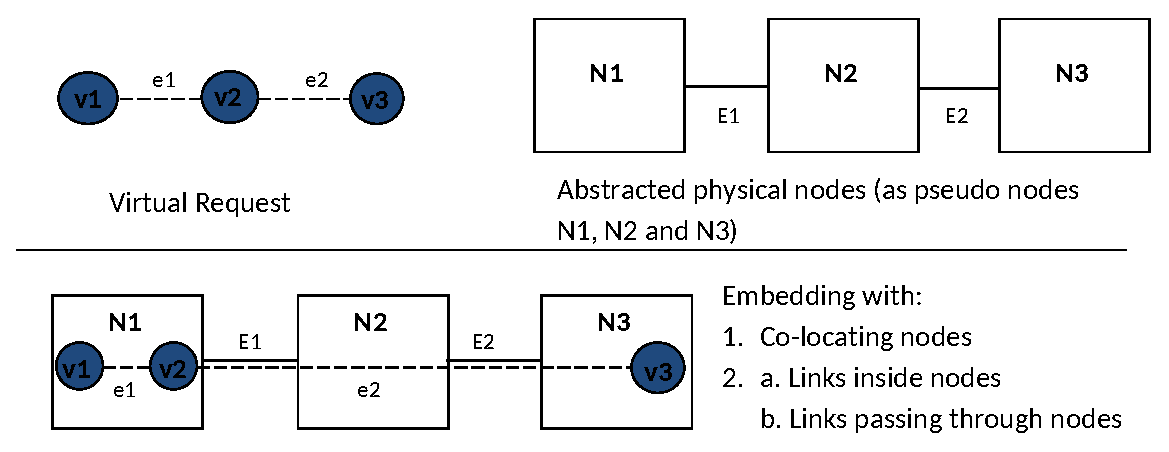
\includegraphics[width=14cm, height=5cm]{modify}
	\caption{Fulfilling requirements with abstraction}
	\label{fig: modify}
\end{figure}


In order to fulfil the requirement of co-locating nodes in a single domain, author proposes the concept of interfaces inside a physical domain. Each link external to a pseudo node is connected to an interface of another pseudo node. Every interface inside a pseudo node is the real interface on the real edge node of a pseudo node to which the external link is connected as shown in figure \ref{fig: modify}. Typically the nodes/routers inside a domain is considered as interfaces. Switching bandwidth between the interfaces of a pseudo node is calculated as actual intra-domain paths between them. As shown in the figure (\ref{fig: modify}), physical topology is abstracted as a pseudo graph on which existing embedding algorithms can be applied. A VN request graph is divided into sub graphs and each sub-graph is assigned to each domain. On receiving the VN sub-graph corresponding operator embeds the sub-graph at the domain level. \newline

The level of abstracting physical network is important to decide the type embedding solutions we obtain. Lower level of abstraction leads to decreased embedding speed because large amount of information about the physical resources is to be processed. And higher level of abstraction results in less efficient solution which are far realistic. Inaccuracy in the abstraction of physical domains at multi-domain orchestrator level also leads to failed VN embedding.\newline

As explained earlier, EdWiN formulation is modified to include the interfaces inside a domain. Switching of networks enables consumption of transformed resources for forwarding nodes. This can be realized with the help of interfaces inside the domains. Interfaces can also be used to realize resources consumption while embedding links on the pseudo nodes. This is called as internal switching. Also by introducing the concept of interfaces we can keep an account of the internal bandwidth of of physical domains. Figure \ref{fig: sw_model} compares old switching model and the proposed switching model that uses interfaces. The left side hexagon represents old switching model of a node $n_{i}$ where as right side hexagon depicts a new switching model with interfaces (p, q in the figure). 
\begin{figure}[h]
	\centering
	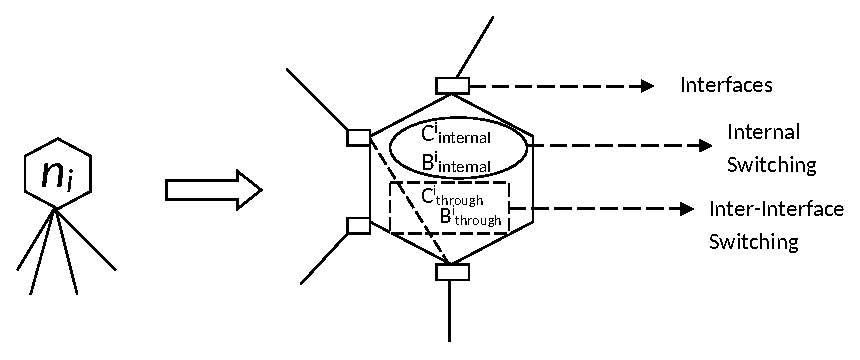
\includegraphics[width=12cm, height=4cm]{sw_model}
	\caption{Switching Model}
	\label{fig: sw_model}
\end{figure}

Now, here we introduce the basic graph models and the modified formulation of EdWiN to support multi-domain embedding. Basic model for the physical network graph and VN request graph is derived directly from EdWiN in the same format (substrate model and vn request model) hence equations Eq. (5) to Eq. (7) remains same.

\begin{enumerate}[label=(\Alph*)]
\item  Formulation for Interfaces: 
	
In EdWiN project, a physical vertex was a simple node having compute, storage and memory resources without the interfaces inside it. But introduction of interfaces inside a physical vertex as depicted in the figure \ref{fig: sw_model} requires a new variable $I_{i}$ representing set of interfaces of a physical node i. Hence,
\begin{itemize}
\item Every physical node $n_{i}$ where $i \epsilon\; \{1..N\}$ (N is set of physical nodes) now has a set of interfaces $I_{i}$.
\item Each interface of a node  $n_{i}$ is given by  $n_{i_{p}}$ where  $p \epsilon \; \{1...I_{i}\}$.
\end{itemize}

\item Links:

In EdWiN, links are represented as a pair $(n_{i}, n_{j})$ with $i, j \epsilon \; \{1...N\}$. With the introduction of interfaces, links are now characterized by $(n_{i_{p}}, n_{j_{q}})$, which says a link exists between interface 'p' of node 'i' and interface 'q' of node 'j'.
	
The boolean variable $x^{gk}_{i_{p}j_{q}}$ represents bandwidth allocated for the virtual link of k-th sub-graph of g-th request on the physical link $l_{i_{p}j_{q}}$. Therefore,
\begin{equation}
\begin{split}
x^{gk}_{i_{p}j_{q}} \epsilon \; \{0, 1\} \; \forall i, j \epsilon \;\{1..N\}; \; p \epsilon \;\{1..I_{i}\}; \; q \epsilon \;\{1..I_{j}\}
\end{split}
\end{equation}
where $x^{gk}_{i_{p}j_{p}} = 0 \; \forall i \epsilon \;\{1..N\}; \; p \epsilon \;\{1..I_{i}\}$

\item Nodes: 

This section introduces formulation that satisfies the requirements mentioned earlier while introducing interfaces concept. That is formulation for 
\begin{enumerate}
\item Resource Transformation and Forwarding: As we know, $B_{ij}$ is the bandwidth capacity of a link connecting the nodes 'i' and 'j'. Now the variable  $B_{i_{p}j_{q}}$ represents bandwidth between the interfaces 'p' and 'q' of a pseudo node $n_{i}$ where $p,q \epsilon \{1...I_{i}\}$. Allocating bandwidth between any interfaces leads to resource consumption. Such resource consumption (compute, storage and memory) is expressed in term of functions $\{C_{through}^{i}$, $M_{through}^{i}$, $S_{through}^{i}\}$. For compute resource, formulation is given by:
\begin{equation}
\begin{split}
C^{i}_{through} =  f_{C^{i}_{through}} \big( \sum_{g=1}^{G} \sum_{k=1}^{k_{g}} \sum_{p=1}^{I_{i}} \sum_{q=1}^{I_{i}} b_{g_{k}}x_{i_{p}j_{q}}^{g_{k}}\big) 
\end{split}
\end{equation}

Similar equations can be derived for  $M_{through}^{i}$ and $S_{through}^{i}$. In the paper all these functions $f_{C^{i}_{through}}$, $f_{M^{i}_{through}}$ and $f_{S^{i}_{through}}$ are replaced by one single function 'f' as $1/\beta$ i.e.
\begin{equation} \label{c-i-through}
\begin{split}
C^{i}_{through} = \big( \sum_{g=1}^{G} \sum_{k=1}^{k_{g}} \sum_{p=1}^{I_{i}} \sum_{q=1}^{I_{i}} b_{g_{k}}x_{i_{p}j_{q}}^{g_{k}}\big)/\beta, \beta \geq 1
\end{split}
\end{equation}

$\beta$ determines the influence of allocated link with the resources of the node that link passes through. 
\item Resource Transformation, Internal Bandwidth: The interfaces are used only when a physical node acts as forwarding node on the embedding path. While embedding if two connected virtual nodes are embedded on same physical node, then those virtual nodes will not only consume resources but also consume extra resource for the connection between them. This extra resource consumption is given by $r^{i}_{internal} = \{C^{i}_{internal}, M^{i}_{internal} , S^{i}_{internal} \}$ where:
\begin{equation} \label{ci-intern1}
\begin{split}
C^{i}_{internal} = f_{C^{i}_{internal}} \big( \sum_{g=1}^{G} \sum_{k=1}^{k_{g}} y^{i}_{s_{g_{k}}} y^{i}_{d_{g_{k}}} b_{gk}\big)
\end{split}
\end{equation}

Similar equations are derived for  $M^{i}_{internal}$ and $S^{i}_{internal} \}$. In order to make these functions linear, a single function is used. Hence above equation becomes:
\begin{equation} \label{ci-intern2}
\begin{split}
C^{i}_{internal} = f_{C^{i}_{internal}} \big( \sum_{g=1}^{G} \sum_{k=1}^{k_{g}} y^{i}_{s_{g_{k}}} y^{i}_{d_{g_{k}}} b_{gk}\big)/\alpha, \alpha \geq 1
\end{split}
\end{equation}
The equations Eq. (\ref{ci-intern1}) and Eq. (\ref{ci-intern2}) are not linear and convex. To linearise them, $ y^{i}_{s_{g_{k}}}$ and $y^{i}_{d_{g_{k}}}$ are replaced by $z^{i}_{g_{k}}$. Boolean variable $z^{i}_{g_{k}}$ is such that:
\begin{equation} 
\begin{split}
z^{i}_{g_{k}} \geq y^{i}_{s_{g_{k}}} + y^{i}_{d_{g_{k}}} -1, \; z^{i}_{g_{k}} \leq y^{i}_{s_{g_{k}}}, \; z^{i}_{g_{k}} \leq y^{i}_{d_{g_{k}}}
\end{split}
\end{equation}
\item  Intra-node Bandwidth models: Here bandwidth limit for intra-node bandwidth consumption is introduced. Figure \ref{fig: bw_model} depicts two bandwidth models used in the work. In 'Common Bandwidth Model' there exists single bandwidth value $B_{i}$, between all the interfaces. Since the bandwidth is shared by all the interfaces, bandwidth consumption in any of the interfaces reduces bandwidth availability for all the interfaces by the amount consumed. Hence $B_{i}$ is given by:
\begin{equation} 
\begin{split}
B^{Available}_{i} = B^{total}_{i} -  \sum_{g=1}^{G} \sum_{k=1}^{k_{g}} \sum_{p=1}^{I_{i}} \sum_{q=1}^{I_{i}} \{x_{i_{p}j_{q}}^{g_{k}} + x_{i_{q}j_{p}}^{g_{k}}\}
\end{split}
\end{equation}
\begin{figure}[h]
	\centering
	\includegraphics[width=8cm, height=3cm]{bw_model.jpg}
	\caption{Switching Model}
	\label{fig: bw_model}
\end{figure}

In 'Independent Bandwidth Model' every pair of interfaces inside a pseudo node 'i', have their own bandwidth which is independent of resource consumption between any other pairs of interfaces. Such bandwidth $B_{i_{p}i_{q}}$ is given by:
\begin{equation} 
\begin{split}
B^{Available}_{i_{p}i_{q}} = B^{total}_{i_{p}i_{q}} -  \sum_{g=1}^{G} \sum_{k=1}^{k_{g}} \{ x_{i_{p}j_{q}}^{g_{k}} + x_{i_{q}j_{p}}^{g_{k}}\}
\end{split}
\end{equation}
\end{enumerate}
\item  Capacity Constraints: 

The bandwidth allocated on each link must be less than the link's capacity. That is $\forall i, j\epsilon \; \{1...N\}, ;\ i \neq j; \; p = 1...I_{i}; \; q = 1...I_{i}$
\begin{equation} \label{bw_cons}
\begin{split}
 \sum_{g=1}^{G} \sum_{k=1}^{k_{g}} b_{g_{k}} \big(x_{i_{p}j_{q}}^{g_{k}} + x_{j_{q}i_{p}}^{g_{k}}\big) \leq B_{i_{p}j_{q}}
\end{split}
\end{equation} 
where $B_{i_{p}j_{q}} = B_{j_{q}i_{p}}$. This equation is valid for both inter-node $(i\neq j)$ and intra-node  $(i= j)$ bandwidth constraint.\newline

The compute capacity required by the virtual node must be less than the compute capacity available on the physical node. Thus,
\begin{equation} \label{cpu_cons}
\begin{split}
\sum_{g=1}^{G} \sum_{k=1}^{K_{g}} \big( C_{s_{gk}} U_{s_{gk}}  y^{i}_{s_{gk}} +  C_{d_{gk}} U_{d_{gk}} y^{i}_{d_{gk}} \big) + C_{internal}^{i} + C_{through}^{i} \leq C_{i} 
\end{split}
\end{equation} 
where \newline

$U_{s_{gk}} = \begin{cases}
0, & \text{if }  \exists k' < k: v_{s_{gk}} \equiv v_{s_{k'g}} \text{or } v_{s_{gk}} \equiv v_{d_{k'g}} \\
1, & \text{ otherwise} \\
\end{cases}$	
		
$U_{d_{gk}} = \begin{cases}
0, & \text{if }  \exists k' < k: v_{d_{gk}} \equiv v_{s_{k'g}} \text{or } v_{d_{gk}} \equiv v_{d_{k'g}} \\
1, & \text{ otherwise} \\
\end{cases}$	


where 'v' represents virtual node and $\equiv$ means "is same as". And the parameters $U_{*_{gk}}$ avoids same virtual node to act as source and destination node for different 'k' sub-graphs. Equation similar to Eq .\ref{cpu_cons} can be derived for other resources like memory and storage.  
\item Topology and Embedding Constraints: 

For a successful VN embedding: 
\begin{itemize} 	
\item For each node,inter-flow bandwidth constraint must be fulfilled. Thus $\forall n = 1...N $
\begin{equation} \label{tec}
\begin{split}
\sum_{p=1}^{I{n}} \bigg\{ \sum_{j=1}^{N} \sum_{q=1}^{I_{j}} x^{g_{k}}_{n_{p}j_{q}} - \sum_{i=1}^{N} \sum_{q=1}^{I_{j}} x^{g_{k}}_{i_{q}n_{p}}\bigg\} = y_{s_{g_{k}}}^{n} - y_{d_{g_{k}}}^{n} 
\end{split}
\end{equation} 
	
\item Each sub-graphs source and destination node is embedded once and only if the whole graph of those sub-graphs is embedded. Hence $\forall i =1...N; \;g = 1...G; \;k = 1...k_{g} $
\begin{equation}
\begin{split}
\sum_{i=1}^{N} y_{s_{g{k}}}^{i}  = y_{g},\; \sum_{i=1}^{N} y_{d_{g{k}}}^{i}  = y_{g}
\end{split}	
\end{equation}
\item Since the VN graph is divided into sub graphs based on links, virtual node (source or destination) of one VN sub graph might be part of another VN sub graph. So $ \forall n = 1...N$		
\begin{equation}
\begin{split}
y^{n}_{s_{g_{k}}} =  y^{n}_{s_{g_{k'}}} ;\ if \quad v_{s_{g_{k}}} = v_{s_{g_{k'}}}\\
y^{n}_{d_{g_{k}}} =  y^{n}_{d_{g_{k'}}} ;\ if \quad v_{d_{g_{k}}}= v_{d_{g_{k'}}}\\
y^{n}_{d_{g_{k}}} =  y^{n}_{s_{g_{k'}}} ;\ if \quad v_{d_{g_{k}}}= v_{s_{g_{k'}}}
\end{split}
\end{equation} 
\item If it is stated explicitly that co-location of nodes is not allowed, the separation can be forced by:
\begin{equation}
\begin{split}
y^{n}_{s_{g_{k}}} +  y^{n}_{s_{g_{k'}}} \leq 1 ;\  if \quad v_{s_{g_{k}}} = v_{s_{g_{k'}}}\\
y^{n}_{d_{g_{k}}} +  y^{n}_{d_{g_{k'}}} \leq 1 ;\  if \quad v_{d_{g_{k}}}= v_{d_{g_{k'}}}\\
y^{n}_{d_{g_{k}}} +  y^{n}_{s_{g_{k'}}} \leq 1 ;\  if \quad v_{d_{g_{k}}}= v_{s_{g_{k'}}}
\end{split}
\end{equation} 
\end{itemize}
\item Intra-node Flow Constraints: For intra-node flow constraints, flow equation around each interface is required. For this new equation the variables $y^{i_{p}}_{s_{g_{k}}}$ and $y^{i_{p}}_{d_{g_{k}}}$ are used,whose value becomes 1 when gk-th source (destination) node uses port 'p' of the node 'i'. The equation is given by $\forall n-1..N, \; p=1.. I_{n}$:
\begin{equation}
\begin{split}
 \sum_{j=1}^{N} \sum_{q=1}^{I_{j}} x^{g_{k}}_{n_{p}j_{q}} - \sum_{i=1}^{N} \sum_{q=1}^{I_{i}} x^{g_{k}}_{i_{q}n_{p}} + 
 \sum_{q=1}^{I_{n}} x^{g_{k}}_{n_{p}n_{q}} -  \sum_{q=1}^{I_{n}} x^{g_{k}}_{n_{q}n_{p}} = y_{s_{g_{k}}}^{n_{p}} - y_{d_{g_{k}}}^{n_{p}} 
\end{split}
\end{equation}
Also to ensure, in any pseudo node only one interface is used as sourceor destination node for a link:
\begin{equation} \label{tec1}
\begin{split}
\sum_{p=1}^{N} y_{s_{g_{k}}}^{n_{p}} = y_{s_{g_{k}}}^{n_{p}}, \; \sum_{p=1}^{N} y_{d_{g_{k}}}^{n_{p}} = y_{d_{g_{k}}}^{n_{p}}
\end{split}
\end{equation}
\item Goal Function:

Here formulation for maximizing the goal function is defined.
\begin{equation}
\begin{aligned}
w\sum_{g=1}^{G} y_{g} &- \sum_{g=1}^{G} \sum_{k=1}^{K_{g}}  \sum_{i=1}^{N} \sum_{p=1}^{I_{i}} \sum_{\substack{j=1 \\ j\neq i}}^{N} \sum_{q=1}^{I_{j}} b_{g_{k}}  x^{g_{k}}_{i_{p}j_{q}}\\ &- (1+\gamma/\beta) \sum_{g=1}^{G} \sum_{k=1}^{K_{g}}  \sum_{i=1}^{N} \sum_{p=1}^{I_{i}} \sum_{q=1}^{I_{i}} b_{g_{k}}  x^{g_{k}}_{i_{p}i_{q}}\\ &- \gamma/\alpha \sum_{g=1}^{G} \sum_{k=1}^{K_{g}}  \sum_{i=1}^{N} b_{g_{k}} z_{g_{k}}^{i} 
\end{aligned}
\end{equation}

where $\gamma = \frac{\text{percentage of free links in substrate}}{\text{percentage of free node resources in substrate}}$ \newline

The objective here is to maximize successful embeddings. The first term ensure that the embedding succeeds. The variable 'w' signifies that the success of the request is more or equally important compared to rest of maximization term. The second term tries to minimize the consumption of bandwidth on the link connecting two different physical domains. Similarly the third term tries to minimize amount of internal bandwidth allocated to virtual links inside a physical domain. The "1" in the co-efficient $(1+\gamma/\beta)$ represents inter-node bandwidth used while $\beta$ in $\gamma/\beta$ stands for compute resource used. And $\gamma$ is used to balance the utilization of links vs nodes while embedding links. The last term is used to minimize the compute
resources used while embedding links into nodes. $\gamma$ is again used to express the relative cost of nodes as compared to links.
\end{enumerate}

The formulations are tested by running a simulation tool. As it is known by now, the embedding is performed in two rounds. In the first round, embedding is done over the pseudo nodes and in the second round embedding is performed inside domain represented by a pseudo node independent of first round. Embedding sub-graphs is considered only if the whole VN request graph is embedded. For simulation, the substrate topology contains two layers. First layer is the inter-domain topology which involves multiple domains interconnected and abstracted as pseudo nodes. Second layer is intra-domain layer which involves multiple nodes interconnected in every pseudo node of the first layer topology. 

\hspace*{1cm}Formulation presented in this work with modification to EdWiN resulted in improved success rates of embedding. For a single physical substrate with 100 nodes, the proposed algorithm takes 50s to embed. But for a physical substrate of 10 pseudo nodes with 10 nodes per pseudo node, it takes one-tenth of a second. This speed up in embedding comes with loss of success rates. But 50 second wait time for embedding one VN request in a physical substrate of 100 nodes indicates the need for multi-domain orchestrator. The results clearly shows the effect of network abstraction and level of exposing information by the topologies. With less information exposed of high level of abstraction, algorithm results in inaccurate allocation of resources. When more information about the resources of a physical domain is exposed to the orchestrator, the rate of acceptance of VN request increases but consuming more time. The increase in time with increase in VN acceptance and increase in information exposure signifies a balance is required between information exposure and solution accuracy. This work makes effort in showing the trade-off between inaccurate exposure of information to multi-domain orchestrator and accurate solution of mapping VNs. \newline

This work presented an flexible approach for VN embedding in multiple domains. It also presented a way for abstracting domain information to appear as flat infrastructure, so that existing embedding algorithms can be reused. It introduced possibility of co-locating virtual nodes. An extension to this work is Distributed Brokering Architecture in which an operator is able to request its peer operators to embed part of VN request that cannot be fulfilled by itself. So that orchestrator can retry the failed VN on different operators except where it failed. The thesis work puts effort in realizing the extension just mentioned i.e Distributed Brokering Architecture. 




Add other papers from Ines Houidi, also just look at people who referred to the edwin and multi operator paper. Provide their high level details (important for your thesis too), explain broker and orchestrator for recursive and multi-domain, Explain MCF. 
MD domain--------------------End of state of art



\newpage
\section{Approach}
In this section, we present approaches used for solving the problem statement mentioned in the introduction part. All the previous algorithms for multi-operator embedding requires topology and resource information of each underlying operator domains. Knowing operator's topology details or capacity details is very crucial for embedding in multiple domains. Embedding algorithm needs to know minimum details of the participating topologies or resource information for selecting suitable physical resources for every VN request. With all the necessary information about each participating topologies it is easier and less time consuming for an orchestrator to provide an accurate embedding solution. \newline

Current approaches provide embedding solutions by assuming every operator exposes their private topology to the orchestrator entity which runs the embedding algorithm. The problem with such solutions is that in the real world, operators may not want to expose their topology details to any other operators. Many operators are reluctant to share their internal working topology, even in the abstracted form, as the topology details are paramount to to their operational success. The high level topology abstraction, if exposed by the operators, results in inefficient embedding solutions, as the algorithms will fail to calculate anything accurately. With this reluctance of exposing topology details, such solutions are very difficult to implement in the real world.\newline  
\begin{figure}[h]
	\centering
	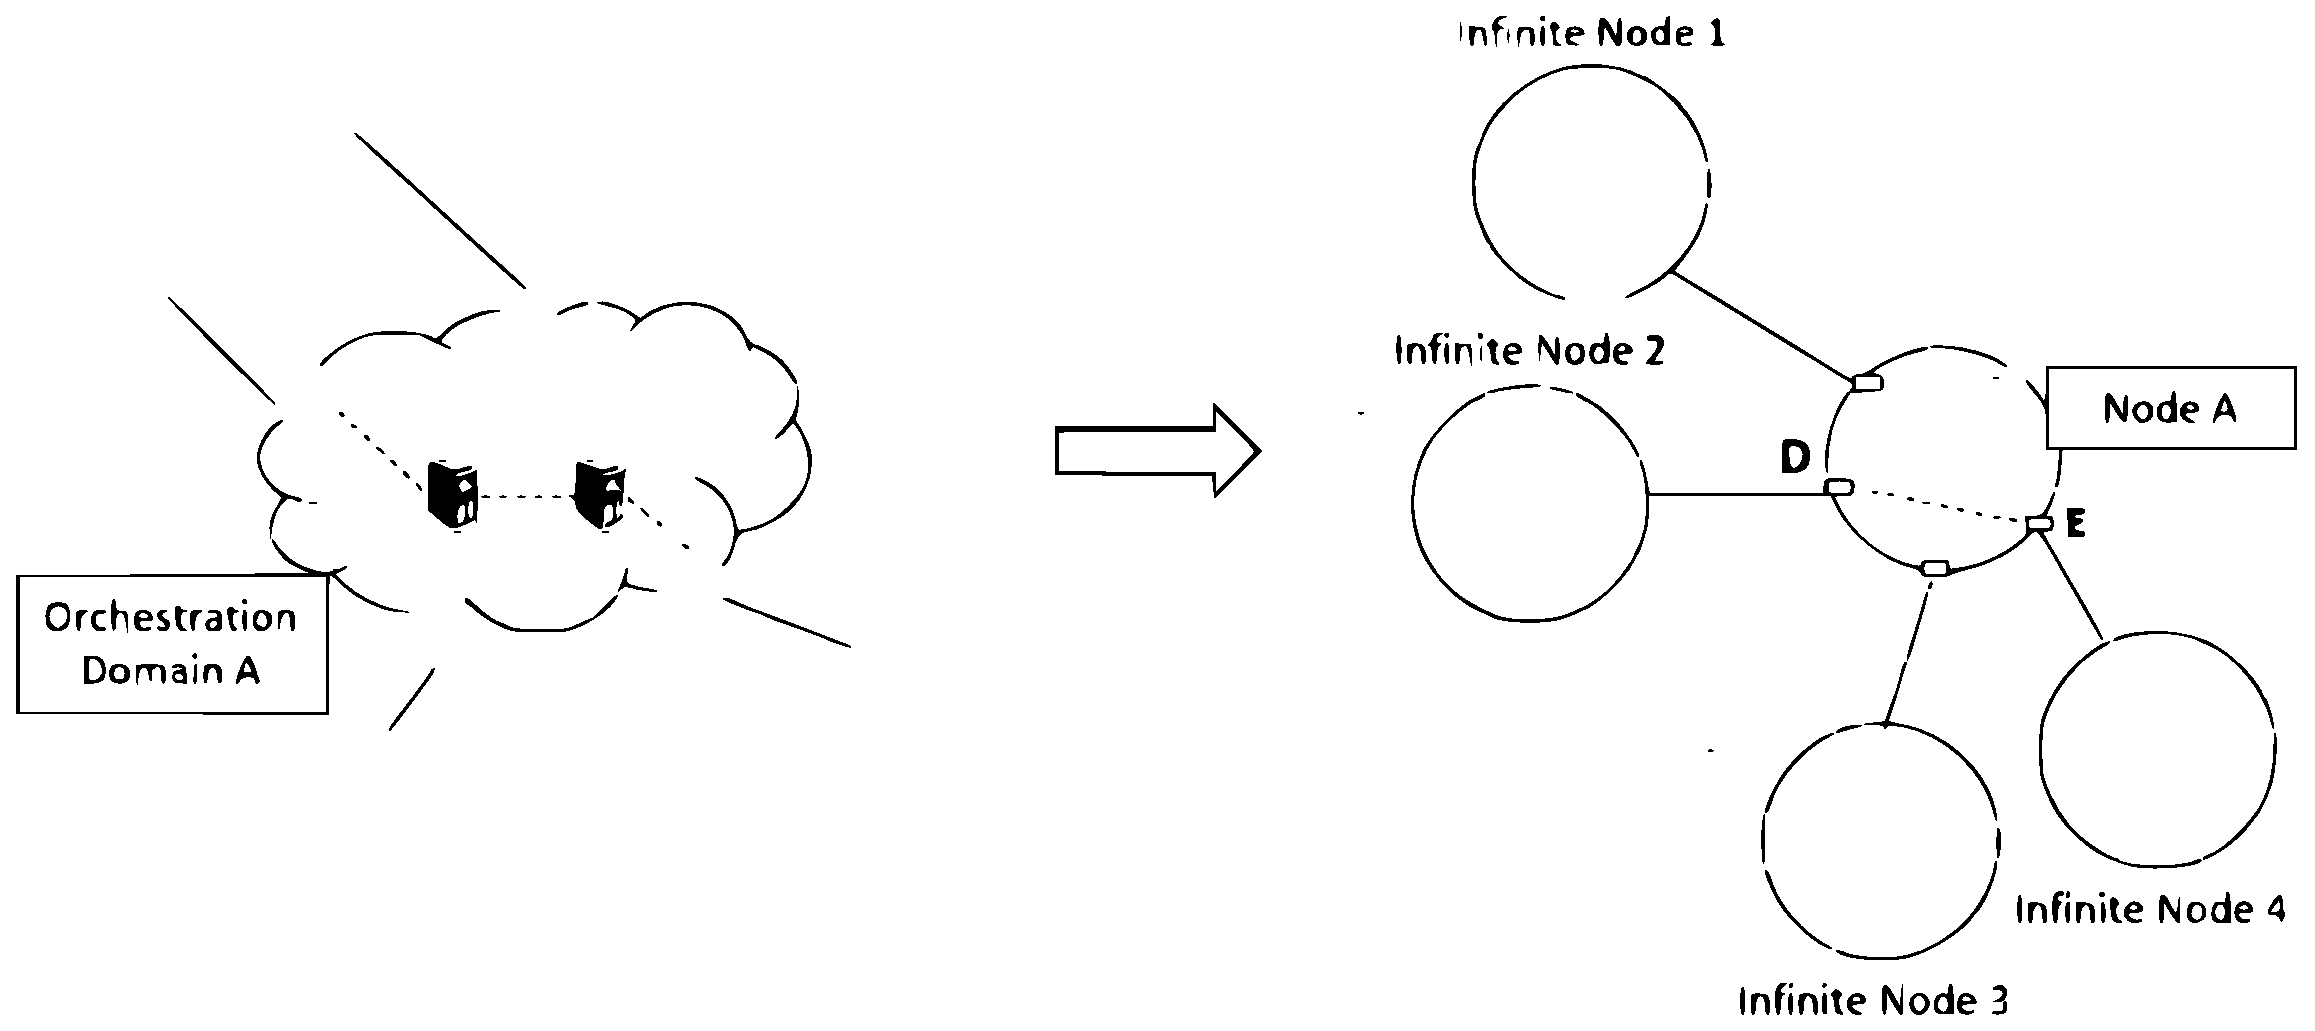
\includegraphics[width=15cm, height=7cm]{Part_embed}
	\caption{Partial Embedding}
	\label{fig: Partial_Embedding}
\end{figure}

Here we propose a solution where operators does not need any information about the topologies of other operators. We propose an architecture where an operator instead of exposing its topology details, shares partial services/VN request that cannot be served by itself to other operators. An operator upon receiving a VN request calculates part of the request it can host and part of the request it cannot embed. Other operators can then evaluate if they are capable of hosting the partial VN request shared by other operator. By this way, an entire VN request can eventually be hosted without the need of topology details from every operator. To support this, we present ILP model where an operator can evaluate from a VN request, the part that it can host and the part that it cannot host.\newline

Consider a scenario depicted in the figure .\ref{fig: Partial_Embedding} where the physical domains are abstracted as nodes. In the figure node A represents operators own node which receives virtual network requests from the customer. The main idea of this work is that the operator that receives the request (operator A) must  divide the service request into a part that can be hosted by the operator himself and another that might be hosted by other  operators. The part that cannot be hosted by the operator is exposed in an external database to which other operators can subscribe. Other operators may then internally evaluate if it can support this partial request. If they can then a negotiation procedure may take place to support the entire request. This way none of the operators need to expose their topologies to each other.\newline

As we mentioned earlier, orchestrator should be able to calculate the part of VN request it can serve. The partially non-embedded part of the request may then be sent to an external database which can be accessed by other operators. The other operators can periodically check this database to see whether they can satisfy the request partially or completely. Some cases the external database may belong to third party broker. The following section provides brief picture on the system required to achieve the above mentioned goals. For this we define important components that are essential for every domains participating in the embedding process. The figure (fig .\ref{orch}) represents basic concept behind an orchestrator, that is responsible for managing and serving incoming VN requests. \newline
\begin{figure}[h]
	\centering
	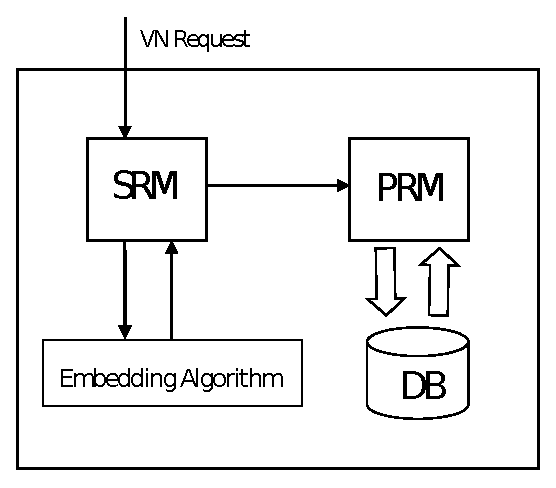
\includegraphics[width=10cm, height=7cm]{orch}
	\caption{Orchestrator A}
	\label{orch}
\end{figure}

The orchestrator has these main components:

\begin{enumerate}
\item  Service Request Manger (SRM): The SRM is responsible for calculating the partial request that it's own domain can fulfil with the help of embedding algorithm. SRM receives VN request and feed it to the 'embedding algorithm'. The algorithm performs mapping based on the objective function defined by the operator.
	
\item Pending Request Manager (PRM): This component receives either a part of VN request that failed in embedding or a whole VN request that failed to embed. In case of failed part of VN, PRM stores failed partial VN request into database. The PRM can be configured to apply some abstraction rules to the separated VN request (partial non-embedded request) received from SRM. 

\item Databases: Orchestrator maintains two databases. The first database stores partial VN that succeeded in the local embedding and second stores failed partial VN for further processing. These two databases are crucial for complete embedding of a VN request as they together contain complete details of a VN request.	
\end{enumerate}
 
Now let us understand the operation of the orchestrator and its components in detail. The following flow charts (fig .\ref{fl}) explains how an VN request is embedded by sharing its parts between different domains. Consider two orchestrating entities Orchestrator A and Orchestrator B participating in the embedding process. The SRM component of the orchestrator A receives a VN request. The embedding algorithm is applied to this VN request to check whether local embedding is possible, i.e whether the VN can be embedded completely on the orchestrator domain A. If local embedding is possible then embedding is considered successful and orchestrator starts processing the next VN request. In case of failed local embedding, SRM with the help of the algorithm, separates the VN request into partial VN requests. The partial VN request may be part of VN request that failed to embed locally or the whole VN request that also failed to embed locally. In both the cases, partial requests are sent to the pending request manager (PRM) of that orchestrator.\newline

The PRM component of an orchestrator saves the non-embedded part of VN request into a database which can be accessed by other operators (fig .\ref{fl}(a)). In order to notify other operators about the saved partial VN, orchestrator can implement a publish/subscribe system or a request crawler which periodically checks other orchestrator's PRM for new partial VN offers. Once the orchestrator B come to know about the partial VN offers, it contacts administrator of the orchestrator A with the corresponding partial VN details. If both orchestrator negotiates on embedding the partial VN request then SRM of orch. B receives the partial VN request. 

After receiving the partial VN request from orch. A, now its orch. B's turn to decide whether it can support the received VN request or not (fig .\ref{fl}(b)). This is done by running the algorithm in orch. B. If orch. B fails to embed the VN request completely, then the embedding is considered as failure and notified to the orch. A. In this case orch. B now starts looking for new partial VNs. If in case orch. B is able to embed the received partial VN completely then the orch. A is contacted saying the VN request can be embedded completely. Now orc. B has to wait until orch. A agrees for complete embedding. If agreement is reached then embedding procedure is continued in both orchestrator for that VN request, if not orch. B stops serving this request an look for new one.

\begin{figure}[h]
	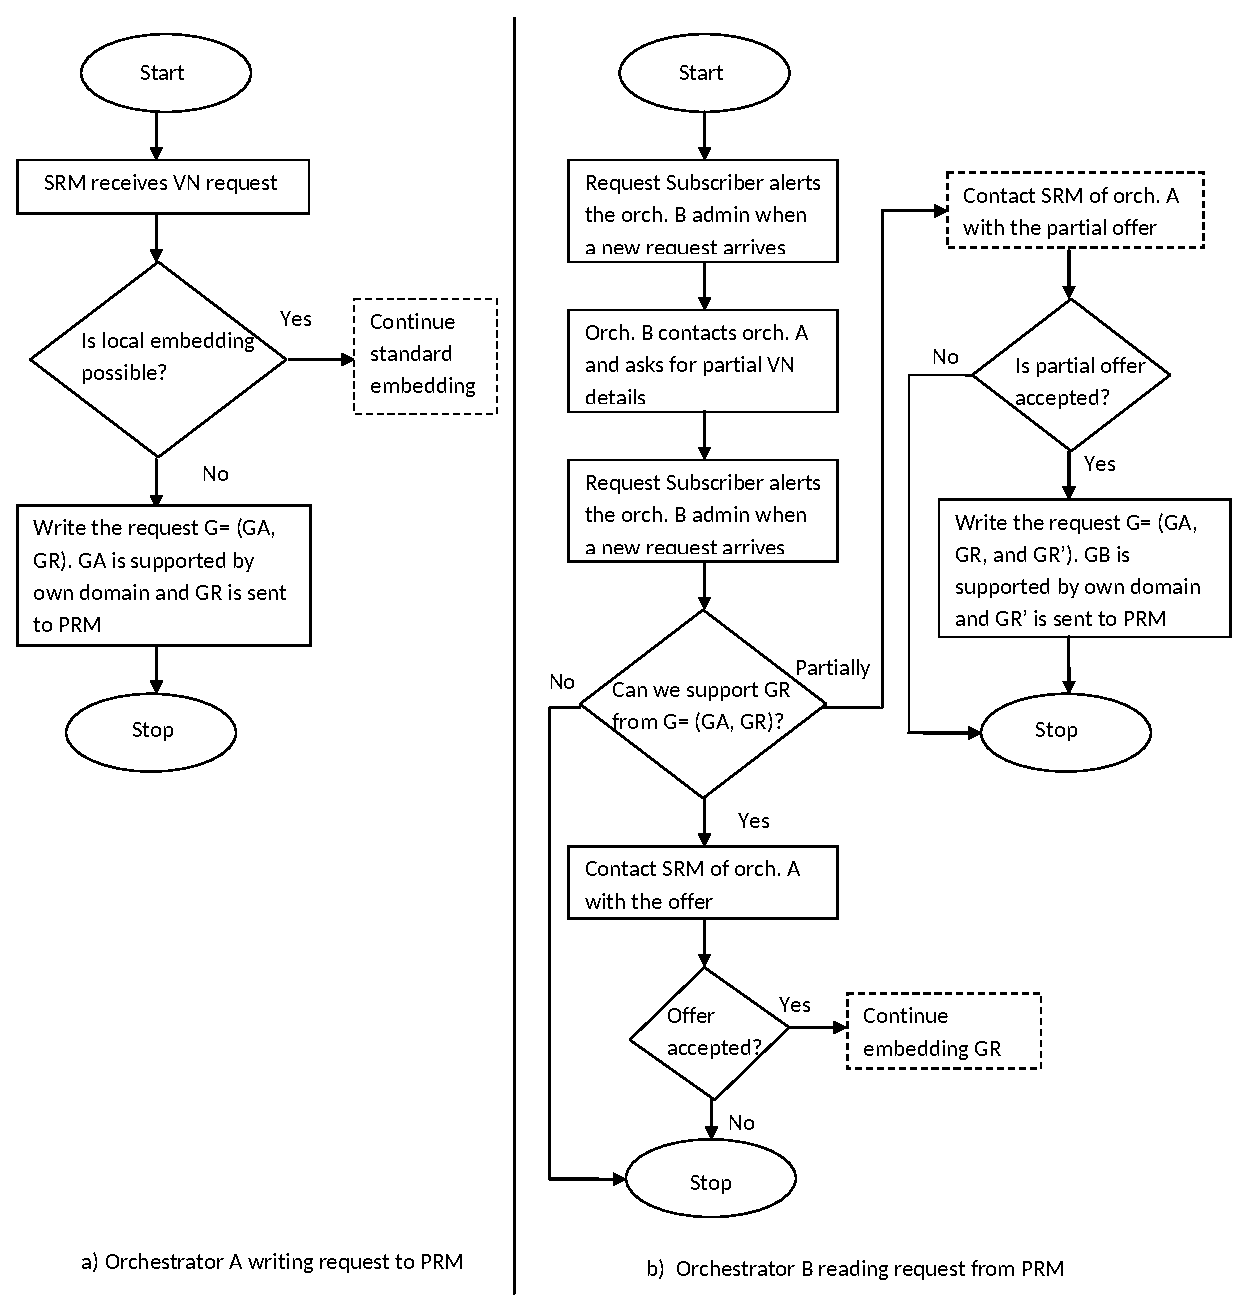
\includegraphics[width=\linewidth]{flowchart}
	\caption{PRM Operations}
	\label{fl}
\end{figure}

In the thesis work, we have used publish/subscribe model for the communication between participating operators. The figure (fig .\ref{pub_sub}) depicts an implementation example for the proposed solution. In general PRM is a concept under each orchestrator domain. But in this implementation, PRM is owned by third party broker and it is accessible by every orchestrator. An operator can access other operator's PRM via HTTP-based RESTful interface. PRM implementation follows publish-subscribe model where orchestrators can subscribe for certain categories of request. In our work, for simplicity we have assigned colours for partial VNs, hence type of the colour is considered as a category. For every partial embedding, the operator creates a partial VN request for the part of the request that failed in embedding. This partial VN request is assigned different colours. Once the partial VN request is generated, the corresponding orchestrator will publish a message in the system. All other orchestrators which have subscribed to a particular colour will receive a message in the form of notification, if a partial VN with the corresponding colour is arrived.

\begin{figure}[h]
	\centering
	\includegraphics[width=\linewidth]{psm1}
	\caption{Publish-Subscribe Model 1}
	\label{pub_sub}
\end{figure}
s
Consider a scenario as in fig .\ref{pub_sub} where three Orchestrators A,B and C are participating in the embedding process. A virtual network request arrives at orch. A with five virtual nodes and four virtual links. Orch. A runs the embedding algorithm to embed this VN request locally in its domain. The embedding solution allows only two virtual nodes to be embedded in the orch. A domain by splitting VN request into two parts. One part of VN that can be embedded locally (red coloured nodes and links) and other (Green coloured nodes  and links) that cannot. In this case orch. A publishes the partial VN request (Green coloured nodes and links) to its PRM with the category "\#GREEN". As we said earlier, PRM can be accessed by any operator, orch. B and orch. C subscribes to the PRM of orch. A for the category "\#GREEN". Since the subscription matches with the published category of VN request, both orchestrators B and C receives notification from orch. A. The notification includes basic information about the partial VN offer and contact details of the publisher. After receiving the notification both orchestrator B and C contact administrator of orch. A requesting the partial VN details. In response to this, orch. A delivers partial VN with the category "\#GREEN" \text{ to} the orchestators B and C. Also, orchestrators can aggregate all the partial VN offers and publish them at once. The receiving orchestrators can select some or all of the partial VNs based on some optimization criteria.\newline

Now at the receiving end of partial VN offers,  the orchestrator's SRM wakes up the system to contact publisher of the partial VN. After negotiating with the publisher, receiving SRM gets complete details of published partial VN offer. SRM runs algorithm to check whether it can locally support the offer in its domain.

\begin{figure}[h]
	\centering
	\includegraphics[width=\linewidth]{psm2}
	\caption{Publish-Subscribe Model 2}
	\label{psm2}
\end{figure}

 Figure (fig .\ref{psm2}) below depicts receiving end of the orchestration. Here both orchestrator B and C receive notification. But only the request of orch. C is accepted by the publisher (orch. A). So orch. C sends an embedding offer saying it can embed the partial VN published by orch. A. If orch. A accepts the request from orch. C then the embedding procedure is continued together by orch. A and C, which results in complete embedding of that VN request. If only part of partial request is supported by orch. C then the remaining part is jointly published to PRM by orch. A and C.

There might be more than one orchestrator that receives the same partial VN offer, in which case, all those orchestrators send embedding requests to the publisher. Multiple offers are queued up in the PRM and it depends on the publishing orchestrator to select one of the requests from the PRM (option A) based on optimization criteria. Embedding offer can be sent via PRM directly (optin B) to the requester also. By this way a VN request can be successfully embedded across multiple domains.\newline

Now we have an overview of embedding process with the help of orchestrator components and pub-sub system. The implementation of the above explained concepts require three main tasks. At first we need to implement embedding algorithm for partial embedding that is able to calculate part of VN that can be embedded locally in operators own domain. We need a communication system between operators for sharing the partial VNs and offers. At last we need a orchestrator that can manage embedding a complete VN request across multiple operator domains. The following sections provides complete details on implementation phase of these three tasks. The tasks also fulfil the requirements of the thesis work mentioned in the introduction part.

\subsection{Requirement I: Partial Embedding}
At first we present the approach for embedding partial services on the physical substrate. To do this, we model an MILP for operator A considering
another operator's topology as a pseudo node with infinite resource. In such scenario, operator A considers other nodes as infinite nodes that can host any number of VNs because they have infinite physical resources. Based on such a model and the knowledge of cost of hosting the other operators, our MILP can try to minimize the total cost of hosting the service over this entire modelled graph. The solution to the MILP results in a proposition of the parts of the VN that need to be placed in Operators A’s network and the parts that cannot be hosted by operator A. The latter part may then be exposed to other operators for evaluation. Therefore instead of exposing individual topology details, operator A exposes the partial VN request. With this approach, operators need not to expose their topology details to others. \newline

This Section provides the solution on how to divide VN request in to parts that are mapped to operators own node and other infinite nodes. We present an ILP formulation that enables the operator to calculate parts of the graph that it can host in its own topology and the part that cannot be served by itself. We name this kind of embedding a VN partially in different domains as "Partial Embedding". We present two albeit related approaches in the following subsections: i) the domain representation where the operators own domain is abstracted ii) where the operators own domain is not abstracted. The
general concept of the solution is the abstraction of each domain to infinite nodes, where in all requests can succeed. However, hosting a request in that infinite node incurs an additional cost factor of $\mu_{d}$ where 'd' is the index of the domain the infinite node represents. The objective then is to minimize the cost. \newline

Self Topology Abstraction: As explained earlier, the domain is itself represented as a pseudo-node and the neighbouring nodes are represented as infinite nodes as shown in \ref{fig: Partial_Embedding} For every operator, his own domain is considered as known domain and other domains as infinite domains. The edge nodes of a pseudo node A (known domain) are connected to infinite nodes. These infinite nodes can host everything. The capacity, bandwidth and other resources are infinite so that these nodes can process every requests and host every virtual network. Embedding virtual request on known node (operator A) incurs cost 'w'. Cost of hosting in infinite nodes is $\mu$ times costlier than hosting on our own node. Typically,  $\mu \geq 1$ but this is not necessary. \newline

Since we use the same basic model presented in the work EdWiN, most of the formulation remains same. Also, we use the concept of abstracting physical nodes and interfaces that we defined in \cite{7116141}. At first, we present basic graph model for physical network and virtual network request which is modified to support partial embedding. Following this, modified formulation for resource constraints and goal function is presented. Hence we consider:

\begin{enumerate}[label=(\Alph*)]
	\item  Basic Model: As defined in EdWiN project, same graph model is used here for both physical network and virtual network request i.e a graph $G= (V, E)$ where 'V' is a set of vertices and 'E' is a set of edges connecting those vertices. Therefore, physical substrate is represented as a graph $G^{S} = (V^{S}, E^{S})$ and virtual request as $G^{V}_{g} = (V^{V}_{g}, E^{V}_{g})$. The physical substrate consists of 'N' number of domains (pseudo nodes and infinite nodes) represented as $V^{S} = \{n_{1},n_{2}...n_{N}\}$. Without loss of generality say for $i = 1...N_{known}$ represent pseudo nodes where the capacity values are known while for $i = N_{known} + 1$ represent infinite nodes. 
	
	\item A price 'p' associated with embedding each of these sub-graphs into physical substrate, which brings in $p_{g}$ price for embedding g-th request.
	
	\item $\mu_{i}^{C}$ is the factor for cost of embedding compute resource in a domain 'i'. Similarly $\mu_{i}^{B}$ is the cost for internal bandwidth allocation in every i-th domain.
	
	\begin{enumerate}
		\item Each physical substrate node $n_{i}$ where $i \epsilon \{1...N\}$ has $I_{i}$ interfaces. Each interface for a node $n_{i}$ is defined as $n_{i_{p}}$ with $p \epsilon \{1...I_{i}\}$. 
		
		\item we formulate link as $\{e_{i_{p}j_{q}} = \{ n_{i_{p}}, n_{j_{q}}\}  \}$ where the link exists between p-th interface of node 'i' and q-th interface of node 'j'. An interface can only be associated to a single link resulting in a maximum of $L \leq N(N-1)$ edges. 
		
		\item Node capacity matrices, for instance: CPU matrix $[ C_{i}]_{i = 1...N}$, where $C_{i} \ge 0 \; \forall i\epsilon \; \{1...N\}$. Identical matrices and equations can be created for other node resources such as storage and memory. 
		
		\item Link capacity matrix $B_{c} = [B_{c_{i_{p}j_{q}}}]$, $ i, j \epsilon \; \{1...N\}$, $ p \epsilon \; \{1...I_{i}\}$, $ q \epsilon \; \{1...I_{i}\}$, where $ B_{c_{i_{p}j_{q}}} \geq 0  \; \forall  i, j \epsilon \; \{1...N\}; e_{i_{p}j_{q}} $ has capacity $B_{c_{ij}}$; We assume $G^{P}$ is an undirected graph, thus $B_{c_{i_{p}j_{q}}} = B_{c_{j_{q}i_{p}}}$. This has no significant impact on the formulation as the directional bandwidth would only introduce one equation in each direction. Note that $B_{i_{p}j_{q}}$ represents the bandwidth available between interfaces p and q belonging to node $n_{i}$.
	\end{enumerate}
	
	\item Virtual Request Model:
	
	VN requests are resolved one by one by embedding G VN requests, $G^{V}_{g} = (V^{V}_{g}, E^{V}_{g})$. We split each VN request $g \epsilon \{1...G\}$ link wise into $g_{k}$ 2-node sub-graphs. The k-th sub-graph, $k \epsilon \{1..g_{k}\}$, of the g-th virtual network is characterized by:
	\begin{enumerate}
		\item Source and Destination nodes  \textit{$v_{s_{g_{k}}}$} and \textit{$v_{d_{g_{k}}}$} with capacity requirements \textit{$C_{s_{g_{k}}}$}, \textit{$S_{s_{g_{k}}}$} and \textit{$C_{d_{g_{k}}}$}, \textit{$S_{d_{g_{k}}}$} respectively.
		\item The requested directional bandwidth \textit{$b_{g_{k}}$}
		\item  Boolean variables
		\begin{equation}
		\begin{split}
		y_{s_{g_{k}}}^{i}=
		\begin{cases}
		1, & \text{if } n_{s_{g_{k}}}\rightarrow n_{i} \\
		0, & \text{if } n_{s_{g_{k}}}\not\rightarrow n_{i} \\
		\end{cases}\\
		y_{d_{g_{k}}}^{i}=
		\begin{cases}
		1, & \text{if } n_{d_{g_{k}}}\rightarrow n_{i} \\
		0, & \text{if } n_{d_{g_{k}}} \not\rightarrow n_{i} \\
		\end{cases}
		\end{split}
		\end{equation}
		where a $\rightarrow$ b implies \textit{a} is embedded in \textit{b} in the solution.
		
		\item The embedding solution for a virtual link is defined by the boolean variable $x_{i_{p}j_{q}}^{g_{k}}$, identifying if bandwidth is allocated on the physical link $l_{i_{p}j_{q}}$ for the k-th sub-graph of the g-th virtual network request. Therefore, 
		\begin{equation}
		x_{i_{p}j_{q}}^{g_{k}} \epsilon \{0, 1\} \;\forall i, j \;\epsilon\; \{1...N\}; p \epsilon \; \{1...I_{i}\}; q \epsilon \; \{1...I_{j}\}\\
		\end{equation}
		where $x_{i_{p}j_{q}}^{g_{k}} = 0, \; \forall i \;\epsilon\; \{1...N\}; p \epsilon \; \{1...I_{i}\}$\newline
		\item Furthermore, allocation of any bandwidth between any pair of interfaces on the same node $n_{i}$ results in a compute resource consumption $\{C^{i}_{through}\}$ is defined same as the equation Eq. \ref{c-i-through}. Similar equation for storage and memory requirement can be formulated. $\beta$ determines the influence of allocated link through bandwidth in the resource of the node it passes through. Typical $\beta$ values for currently available high end router slots can be calculated by assuming that the maximum switching capacity of the slot uses all the resource available therein. Then the ratio of the maximum switching capacity to the maximum supported link bandwidth gives us a good estimate of $\beta$.
		
		\item 	Finally the whole VN request  $G_{g}^{V}, \; \forall g \;\epsilon\; \{1...G\}$, is characterizes by a boolean variable:
		\begin{equation}
		y_{g}=
		\begin{cases}
		1, & \text{if }   G_{g}^{V}\rightarrow G^{P} \\
		0, & \text{if }   G_{g}^{V}\not\rightarrow G^{P} \\
		\end{cases}
		\end{equation}
		
		Intra-node bandwidth model: We are using 'Independent Bandwidth Model' where, between each pair of interfaces in any node i, there is a bandwidth $B_{i_{p}j_{q}}$ that is independent of the consumption between any other pair of resources. Therefore assuming the bandwidth consumption in both directions equally
		\begin{equation}
		B_{i_{p}j_{q}}^{Available} = B_{i_{p}j_{q}}^{total} -  \sum_{g=1}^{G} \sum_{k=1}^{k_{g}}  \{ x_{i_{p}j_{q}}^{g_{k}} + x_{i_{q}j_{p}}^{g_{k}}\}
		\end{equation}
	\end{enumerate}
	
	\item Constraints:
	
	The constraints for the resource allocation are applied only to the known nodes. As infinite nodes are assumed to have infinite resources, these constraints are not applicable to them that is for $i \geq N_{known} + 1$. Hence the previous equation for bandwidth constraint (Eq. \ref{bw_cons}) can be modified as:
	\begin{equation}  
	\begin{split}
	\sum_{g=1}^{G} \sum_{k=1}^{k_{g}} b_{g_{k}} \big(x_{i_{p}j_{q}}^{g_{k}} + x_{j_{q}i_{p}}^{g_{k}}\big) \leq B_{i_{p}j_{q}} \text{ if } i \leq N_{known} \text{ OR } j \leq N_{known}
	\end{split}
	\end{equation} 
	
	For the capacity constraints at the nodes, Eq. \ref{cpu_cons} can be modified as: 
	\begin{equation}  \label{part_cons}
	\begin{split}
	\sum_{g=1}^{G} \sum_{k=1}^{K_{g}} \big( C_{s_{gk}} U_{s_{gk}}  y^{i}_{s_{gk}} +  C_{d_{gk}} U_{d_{gk}} y^{i}_{d_{gk}} \big) + C_{internal}^{i} + C_{through}^{i} \leq C_{i} \;\;\; \forall i \leq N_{known}
	\end{split}
	\end{equation} 
	where \newline
	
	$U_{s_{gk}} = \begin{cases}
	0, & \text{if }  \exists k' < k: v_{s_{gk}} \equiv v_{s_{k'g}} \text{or } v_{s_{gk}} \equiv v_{d_{k'g}} \\
	1, & \text{ otherwise} \\
	\end{cases}$	
	
	$U_{d_{gk}} = \begin{cases}
	0, & \text{if }  \exists k' < k: v_{d_{gk}} \equiv v_{s_{k'g}} \text{or } v_{d_{gk}} \equiv v_{d_{k'g}} \\
	1, & \text{ otherwise} \\
	\end{cases}$	
	
	
	where 'v' represents virtual node and $\equiv$ means "is same as". And the parameters $U_{*_{gk}}$ avoids same virtual node to act as source and destination node for different 'k' sub-graphs. Equation similar to Eq .\ref{part_cons} can be derived for other resources like memory and storage.  
	\item Topology and Embedding Constraints: 
	
	Formulation for topology and embedding constraints remains same as defined in the previous work (\ref{md_monitoring}). Hence the equations Eq .\ref{tec} to Eq .\ref{tec1} remains same and is used in the thesis work as it is.
	
	\item Goal Function:
	
	The goal is to maximize the profit for the operators own domain and to minimize the resource utilization in the infinite nodes. as the cost of embedding is higher in the infinite nodes. Therefore goal function is formulated as:
	\begin{equation} \label{part_enb_goal}
	\begin{aligned}
	\sum_{g=1}^{G} p_{g} y_{g} &- \sum_{g=1}^{G} \sum_{k=1}^{K_{g}}  \sum_{i=1}^{N} \sum_{p=1}^{I_{i}} \sum_{\substack{j=1 \\ j\neq i}}^{N} \sum_{q=1}^{I_{j}} \mu^{B}_{i_{p}j_{q}} b_{g_{k}} x^{g_{k}}_{i_{p}j_{q}}\\ &- (1+\gamma/\beta) \sum_{g=1}^{G} \sum_{k=1}^{K_{g}}  \sum_{i=1}^{N} \sum_{p=1}^{I_{i}} \sum_{q=1}^{I_{i}}  \mu^{B}_{i} b_{g_{k}}  x^{g_{k}}_{i_{p}i_{q}}\\ &- \gamma/\alpha \sum_{g=1}^{G} \sum_{k=1}^{K_{g}}  \sum_{i=1}^{N}  \mu^{B}_{i} b_{g_{k}} z_{g_{k}}^{i} \\ &- \sum_{i=1}^{N} \sum_{g=1}^{G} \sum_{k=1}^{K_{g}} \mu^{C}_{i}  \big( C_{s_{gk}} U_{s_{gk}}  y^{i}_{s_{gk}} +  C_{d_{gk}} U_{d_{gk}} y^{i}_{d_{gk}} \big) + C_{internal}^{i} + C_{through}^{i}
	\end{aligned}
	\end{equation}
\end{enumerate}
where $\gamma = \frac{\text{percentage of free links in substrate}}{\text{percentage of free node resources in substrate}}$ \newline

\hspace*{2cm} The first term ensures that the embedding succeeds with maximized profit for operator's own domain. The variable '$p_{g}$' represents the price for each 'g' VN requests. The rest of the term tries to minimize resource consumption related to the allocation of bandwidth. CPU resources are not considered as they are used in a fixed amount in every request if it were to succeed. The second term tries to minimize the consumption of bandwidth on the link connecting two different physical domains. The bandwidth cost $\mu_{i}^{B}$ associated with each domain 'i' also determines the solution for each VN request. Similarly the third term tries to minimize amount of internal bandwidth allocated to virtual links inside a physical domain. The "1" from the co-efficient $(1+\gamma/\beta)$ represents inter-node bandwidth used while $\beta$ in $\gamma/\beta$ stands for compute resource used. And $\gamma$ is used to balance the utilization of links vs nodes while embedding links. The last term is used to minimize the compute
resources used while embedding links into nodes. The fourth term tries to minimize the compute resource used while embedding links into nodes. And the last term tries to minimize the compute power used for the virtual nodes while mapping onto physical node.\newline

The following section presents details on the experiment set up and in house simulation tool used to implement the proposed algorithm. After that, we present details on the results gathered for the partial embedding process. \newline

Simulations were executed on a server by solving MIP formulation using the Gurobi library running in Java on 4 cores. A fixed substrate topology with 4 different operators is created as shown in the figure \ref{sub_topo}. In this topology, one node is made as a known node (operator's own node) and other nodes as unknown nodes (infinite nodes). Substrate topology has two layers with first layer having inter-operator topology. This layer includes $N_{operator}$ pseudo nodes abstracting the the operators. The second layer is a intra-operator topology consisting of 'N' number of nodes in each pseudo-node or operator domain. Both inter-domain and intra-domain topologies are randomly generated with random resources and random connection between the pseudo nodes. In intra-operator topology, initially each node has random node capacity generated between 50 and 100 units. Link capacity is randomly generated and uniformly distributed between 50 and 100 units. For each operator node (pseudo-node), available node capacity is equal to the summation of the capacity of the node it contains. \newline

In the figure (fig .\ref{sub_topo}) the rectangular boxes represent nodes and the lines represent links connecting different nodes (domains/operators). The node (node Id: 3741663) with dark shade is known node and others (node Ids: 3741664, 3741665, 4281031) are infinite node. Known nodes have finite number of resources, for instance, the known node here has 70 CPU units, 91 memory and 51 storage units. The overall bandwidth capacity of the known node is 320 units. But the infinite nodes have infinite resources with CPU, storage and memory as 100000 units. The external link connecting two pseudo nodes, out of which if one is infinite node, have infinite bandwidth resource. Since we have configured 2 digit numbers for VN resources (CPU, memory, storage), 100000 units is considered as infinite resources. 

\begin{figure}[h]
	\centering
	\includegraphics[width=12cm, height=7cm]{sub_topo.jpg}
	\caption{Substrate Topology}
	\label{sub_topo}
\end{figure}

VN are created by generating virtual network with four virtual nodes as shown in the figure \ref{virt_topo}. The capacity requirements of the virtual nodes and links are integer numbers randomly generated and uniformly distributed, respectively in the range 1 to 100xVNF (Virtual Node Factor) units and 1 to 100xVLF (Virtual Link Factor) units, where VNF, VLF $\epsilon (0, 1)$ are the simulation parameters that define the ease for incorporating virtual nodes in physical nodes and virtual links in physical links. \newline
\begin{figure}[h]
	\centering
	\includegraphics[width=8cm, height=5cm]{virt_topo.jpg}
	\caption{Virtual Network Request Topology}
	\label{virt_topo}
\end{figure}

The following section provides the details on configuring the orchestrator part. Most of the variables defined the formulation are assigned values in this configuration part. A simple GUI is designed to accept values for different variables and provide a visual screens with controls to understand embedding of each VN request.
\begin{figure}[h]
	\centering
	\includegraphics[width=13cm, height=8cm]{config.jpg}
	\caption{Configuration GUI}
	\label{config}
\end{figure}

The cost factors explained in the goal function Eq .\ref{part_enb_goal} can be set using the GUI inputs. GUI (figure .\ref{config}) allows to assign different values for compute cost and bandwidth cost in known nodes and infinite nodes. The cost factors $\mu_{i}^{B}$ and  $\mu_{i}^{C}$ are set keeping the cost for known nodes cheaper compared to the costs for resources in infinite nodes. The configuration GUI for each orchestrator provides option to select more than one known nodes leaving the remaining as infinite nodes by default. The VN requests are generated simultaneously and fed to the embedding algorithm which process the request one by one. After solving the MIP problem, the embedding algorithm embeds the requests characterized by the variable $y_{g} = 1$ by reducing the capacity of the substrate. Every time a VN request is embedded successfully, the resource capacity of the underlying physical domains get decreased by the amount of resources allocated to that VN request. For every VN request, the algorithm while embedding resources in the first level (pseudo-node level) also performs embedding in the domain level (inside domains) simultaneously.\newline

\begin{table}[h]
	\centering
	\caption{Cost Configuration Table}
	\label{cost_table}
	\begin{tabular}{ |p{2cm}||p{5cm}|p{3cm}|} 
		\hline
		\multicolumn{3}{|c|}{Configuration} \\[2ex]
		\hline
		Variable& Description &Value assigned\\[2ex]
		\hline
		$p_{g}$   & Price of g-th VN request & 1000 to 1500 \\[3ex]
		$\mu_{i_{p}j_{q}}^{B}$ &   External link bandwidth cost  & 3   \\[3ex]
		$\mu_{i}^{B}$ & Internal link bandwidth cost for domain 'i' & Known nodes=1, infinite nodes=1\\[3ex]
		$\mu^{C}_{i}$    & Compute cost for each domain 'i' &  Known nodes=3, infinite nodes=5\\[3ex]
		$\alpha$ &   Switching Alpha  & 100\\[3ex]
		$\beta$ &   Switching Beta  & 100\\[3ex]
		\hline
	\end{tabular}
\end{table}
The values for the corresponding cost factors used in the experiment is tabulated (Table \ref{cost_table}). The input textboxes in the GUI corresponds to the rows in the table. For the price '$p_{g}$', value is assigned while generating VN request graph. For $\beta$ and $\gamma$ value is assigned for in the code. Total number of pseudo-nodes, number of nodes inside each pseudo-node and number of nodes in virtual network request can be changed in the simulation code. The dropdown field "Known domains" \text{ in} the GUI accepts multiple input and represents number of known domains. It is possible to select any of the pseudo-nodes in the network. The field "BW Cost-K Domains" \text{ accepts} input for the variable $\mu_{i}^{B}$ (internal link bandwidth cost), but only for selected known nodes. Similarly the field "BW Cost-Inf. Domains" \text{ accepts} input for the variable $\mu_{i}^{B}$ (internal link bandwidth cost), but only for infinite nodes. For the variable $\mu_{i}^{C}$ values in the fields "Compute Cost-K. Domains" \text{ and}  "Compute Cost-Inf. Domains" \text{ are} used for known nodes and infinite nodes respectively. For external links connecting two pseudo-nodes, value from the textbox "Ext-link cost" \text{ is} used. By clicking the run button with all the values assigned, the algorithm starts mapping virtual nodes while displaying visual graphs for physical network and VN request. Simulation also provides visuals of mapping virtual nodes and link on to physical network.\newline

The figure below (Figure .\ref{Partial_embedding}) depicts embedding process with a VN request containing four virtual nodes with node Ids 13541991, 13541992, 83121213 and 83121214. The right-hand side frame shows embedding of these four virtual nodes on to the physical network containing five different domains (pseudo nodes). For the simulation we have selected one pseudo node as known domain (red/dark coloured rectangle). The known domain (node Id: 3741663) has finite number of resources (CPU:270 units, storage:45 units and memory:12) and belongs to the operator where the algorithm is running. Other pseudo nodes except the node: 3741663 is considered as infinite nodes and the resources are set to high numbers (CPU:100000 units, storage:100000 units and memory:100000). Now in this scenario, the orchestrator inputs the virtual network request by splitting them edge-wise sub-graphs. These sub-graphs are embedded one by one according to the formulation we have presented. In the figure, we can see the result of the algorithm showing, the virtual nodes 83121213 and 83121214 are embedded on the known node (3741663) and two other virtual nodes 13541991, 13541992 are not embedded on the known node. The small rectangular boxes overlapping on bigger rectangles represents virtual nodes that are mapped on to the physical domains.

\begin{figure}[h]
	\centering
	\includegraphics[width=\linewidth]{embedding.png}
	\caption{Partial Embedding}
	\label{Partial_embedding}
\end{figure}

This fulfils our first requirement of partial embedding. Now our algorithm is able to decide how many virtual nodes and links can be embedded on the known node and how many cannot, from a single VN request. There are other scenarios where the whole VN request can be embedded in one single known node and whole VN request fails to embed on the known node. Most of the previous algorithms did not allow partial embedding,stating whole VN request fails if any of its nodes and links cannot be embedded. The embedding solution here depends mainly on the embedding cost of different pseudo nodes. This brings in three cases where:
\begin{enumerate}
	\item Embedding cost in Known nodes are cheaper than embedding in infinite nodes: In this case the orchestrator embeds most of the virtual networks in known nodes. After some time VN request gets split between the domains based on the objective set in the goal function. The resources of infinite nodes are used when the known nodes does not have sufficient amount of resources to serve.
	
	\item  Embedding cost in Known nodes are costlier than embedding in infinite nodes: In this case all of the VN requests are embedded only in infinite nodes. None of the request fails because infinite nodes have infinite resource which can serve any number of VN request with any type of resource demands.
	
	\item Cost of embedding in Known nodes and infinite nodes are same: Here VN request is embedded on any domain which has sufficient amount of resources for the VN request. 
\end{enumerate}

Results: 
In our experiment we assigned low embedding costs to known domains and high embedding costs to infinite domains (table .\ref{cost_table}), so that operator's own domain makes high profit by leasing its resources to more number of virtual networks. The results gathered in the experiment shows that, in the beginning our algorithm starts allocating known node's resources to VN requests till there is sufficient amount of resource to embed. After that  
the resources from infinite nodes are used to serve the upcoming VN requests. We run the simulation with 100 virtual network requests with each request having different topology compared to others. Same number of virtual nodes are used for every VN request. Only difference is the connection between the virtual nodes and the resource demand they have. The following results depicts average resource allocation for same set of 100 VN request for 10 different physical network topologies keeping the embedding costs and other parameters same.

\begin{figure}[h]
	\centering
	\includegraphics[width=10cm]{CPU_PE.png}
	\caption{Average CPU Allocation}
	\label{cpu_alloc}
\end{figure}

The figure (fig .\ref{cpu_alloc}) shows the allocation of CPU resource for each VN request. We mainly considered CPU demand and bandwidth demand as VN resource demands. As mentioned earlier each virtual node has CPU demand in the range of 1 to 100xVNF CPU units where VNF is taken as 0.5. Because of the embedding cost in known nodes being cheaper than infinite nodes, the algorithm starts using maximum resource in the known nodes. Also because of higher embedding cost, resource from infinite nodes are only used when there is no sufficient amount resource for a VN. This can be observed from the figure where the entire resource demands from the first few VN requests are served only in known nodes (Red in colour). That is, 100\% of the resource demands from VNs are allocated in the known node. After some time, this percentage gradually decreases because of insufficient resource in known domain. Then the resource from infinite resource are used for next set of VN requests. For instance, after some 25 VN requests, more than 50\% of the resource demand is served by infinite nodes. And when the VN request is nearer to 90 only 20\% of resource demand is served by knnown nodes and remaining 80\% of the resource is allocated in infinite nodes. It can be seen that for most of the VN requests, resource are allocated both in known nodes and infinite nodes which is a clear indication of "Partial Embedding ". \newline

Similar results are obtained for bandwidth allocation for each virtual link of a VN request. When all the virtual nodes are embedded in known nodes, bandwidth for all the virtual links of this VN request is allocated in the same known node. But in case of partial embedding, more bandwidth is allocated altogether in known and infinite nodes than the actual bandwidth demand by the VN request. This is because of a scenario where a 2-node sub-graph is embedded, one virtual node mapped in known node and one in infinite node. In this case the single link connecting these two nodes need to be embedded in both known nodes and infinite nodes. For instance, consider a 2-node graph with virtual link bandwidth demand of 10 units. When one virtual node is embedded in known domain, a virtual link of bandwidth 10 units is also embedded in that known node. For the second virtual node embedded in the infinite node, again a virtual link with 10 bandwidth units is mapped in this infinite node. So two virtual links each of 10 bandwidth units are embedded. The figure (fig .\ref{BW_alloc}) below depicts bandwidth allocation for each VN request in both known nodes and infinite nodes.
\begin{figure}[h]
	\centering
	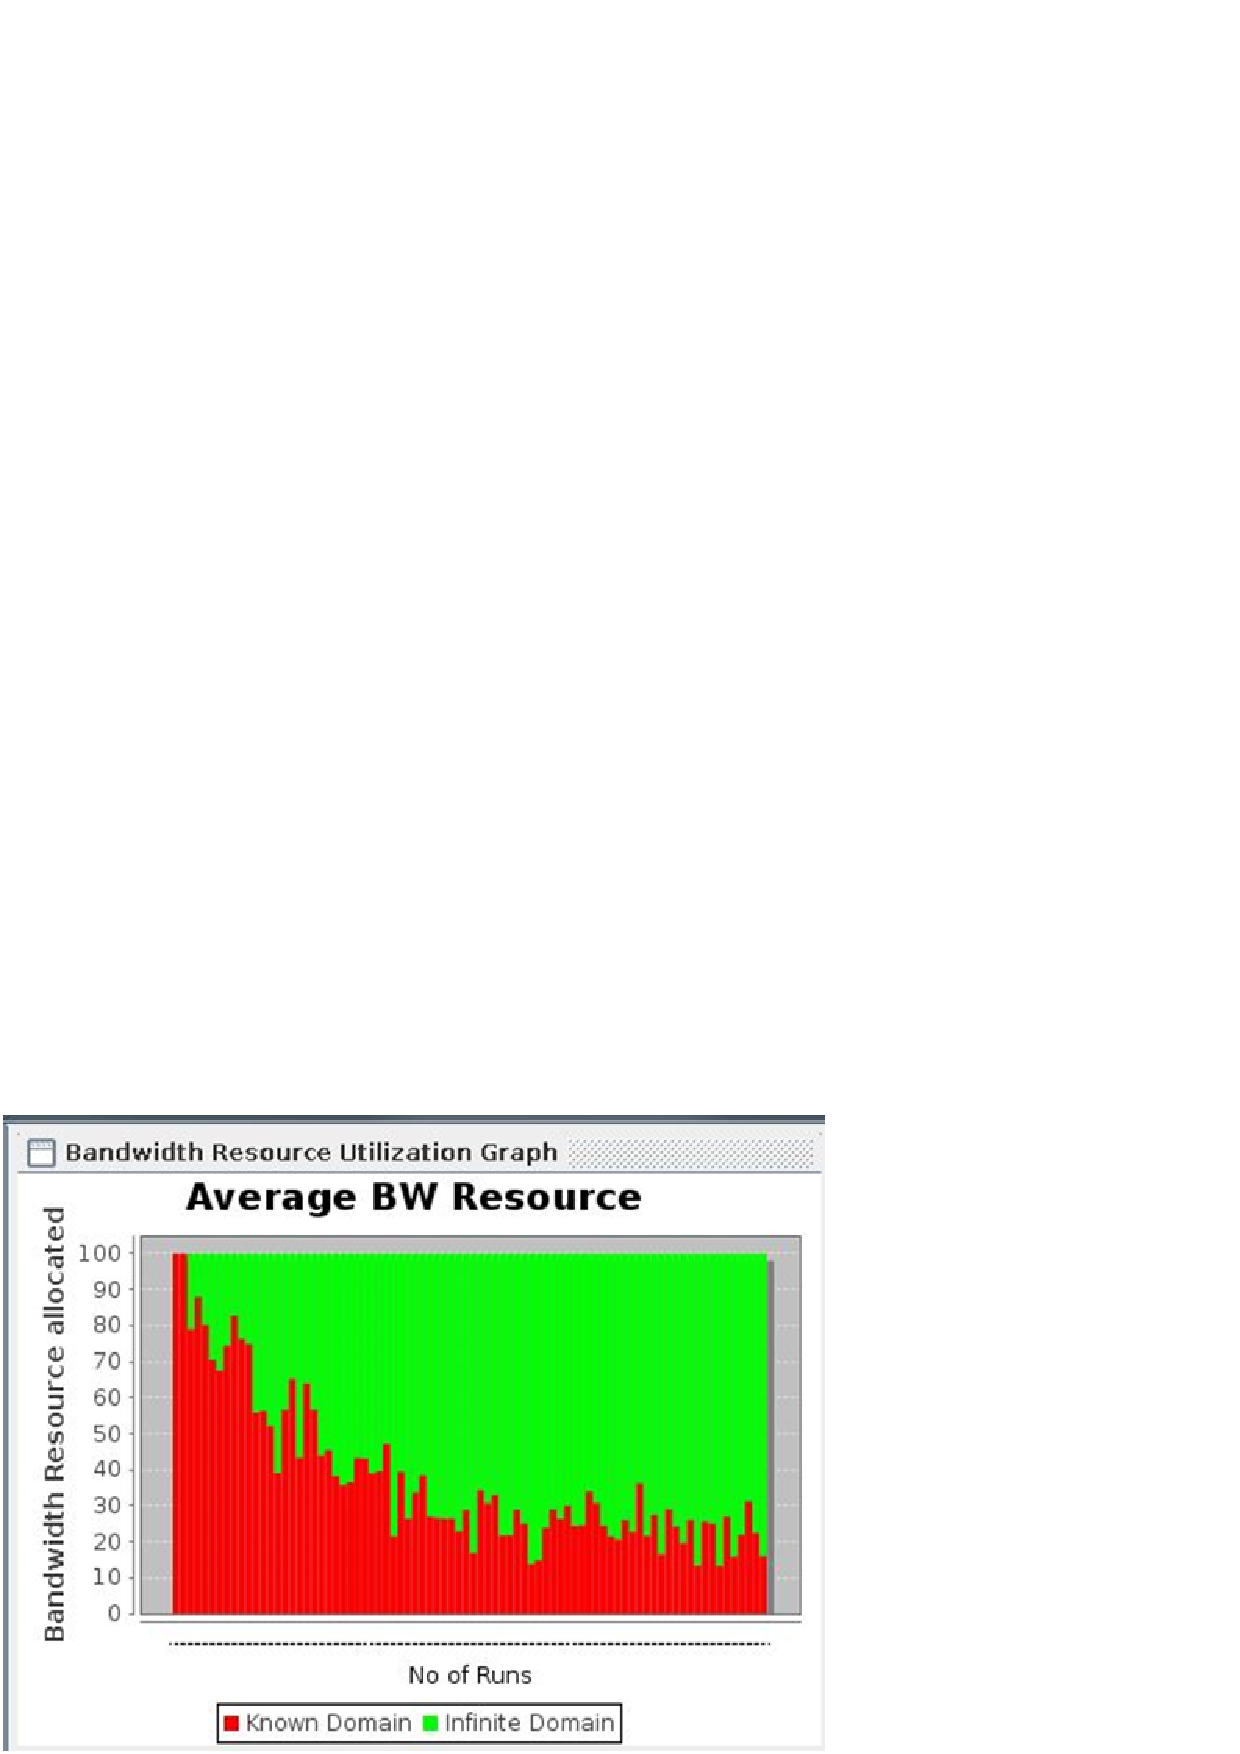
\includegraphics[width=10cm]{BW_PE.png}
	\caption{Average Bandwidth Allocation}
	\label{BW_alloc}
\end{figure}

Another graph below (fig .\ref{resr_consumption}) summarizes resource allocation and how the resources are consumed in known nodes for every VN request. This graph is to show the resource status only in known nodes and resource status of infinite nodes are not considered. The graph has four plots with different colours representing type of resource allocated and consumed. The line with blue colour represents CPU allocation in the known nodes. It clearly shows for the first 2-3 VN requests 100\% of resource demand is served by known nodes. With the increase in incoming VN requests, this blue line gradually decreases. The blue line plot is another way of visualising the graph in fig .\ref{cpu_alloc}. The brown line plot represents bandwidth allocated for every VN request. Same as in the CPU allocation, bandwidth allocation in known nodes also decrease with increase in VN requests. \newline 

\begin{figure}[h]
	\centering
	\includegraphics[width=15cm, height=8cm]{RES_CON_PE.png}
	\caption{Summary of Resource Allocation and Consumption in Known Nodes}
	\label{resr_consumption}
\end{figure}
The remaining two plots represents resource availability in known nodes after serving each VN requests. At first the available resource was full (100\%) till the first VN request is served. The green line plot is for showing remaining CPU capacity of the known node and purple line plot for remaining bandwidth capacity of a known node. It can be observed that maximum CPU and bandwidth resources are consumed for first few VN requests leaving the resource capacity to almost 10\% of the resource the known node had, before embedding any VN request. From the VN request 20 to 80 resource from both known node and infinite nodes are utilized, hence the the remaining resource decrese gradually in known node. The resources of the known node is utilized till it almost becomes 0\%. At this stage, algorithm starts looking at infinite node for upcoming VN requests. 
\newpage
\subsection{Requirement II: }

Starting from partial vn from algo output- nodes links scenarios (few nodes , all nodes of a request), creating partial VN in vnffg format, inserting in db with db script, db pics. why two tables, 
Pub/sub system as per patent----till next page..
after that my work of pub sub and pub sub notif. selecting the peer pip all till page 10.
 
\newpage
\bibliography{biblography} 
\bibliographystyle{ieeetr}

\end{document}
